\chapter{Ridge estimation of the VAR(1) model and its time series chain graph from multivariate time-course omics data \\ {\footnotesize (\textit{Miok, V., Wilting, S. M. and van Wieringen, W. N., Biometrical Journal (2017), 59(1), 172-191})}}
\label{ch3:ragt2ridges}
\chaptermark{Ridge estimation of the VAR(1) model}
\label{chapter:Estimating entropy loss in Gaussian graphical models}
\graphicspath{{Chapter3/Figs/}{Chapter3/Figs/PDF/}{Chapter3/Figs/}}%

Omics experiments endowed with a time-course design may enable us to uncover the dynamic interplay among genes of cellular processes. Multivariate techniques (like VAR(1) models describing the temporal and contemporaneous relations among variates) that may facilitate this goal are hampered by the high-dimensionality of the resulting data. This is resolved by the presented ridge regularized  maximum likelihood estimation procedure for the VAR(1) model. Information on the absence of temporal and contemporaneous relations may be incorporated in this procedure. Its computational efficient implementation is discussed. The estimation procedure is accompanied with an LOOCV scheme to determine the associated penalty parameters. Downstream exploitation of the estimated VAR(1) model is outlined: an empirical Bayes procedure to identify the interesting temporal and contemporaneous  relationships, impulse response analysis, mutual information analysis, and covariance decomposition into the (graphical) relations among variates. In a simulation study the presented ridge estimation procedure outperformed a sparse competitor in terms of Frobenius loss of the estimates, while their selection properties are on par. The proposed machinery is illustrated in the reconstruction of the p53 signalling pathway during HPV-induced cellular transformation. The methodology is implemented in the \texttt{ragt2ridges} R-package available from CRAN.
\\
\\
This chapter was published as:\\
Miok, V., Wilting, S. M. and van Wieringen, W. N. (2017). Ridge estimation of the VAR(1) model and its time series chain graph from multivariate time-course omics data. \textit{Biometrical Journal}, 59(1), 172-191.

\section{Introduction}
Molecular biology aims to unravel the workings of the cell. This amounts to which and how molecules like mRNAs work together. A widely accepted paradigm assumes a modular set-up \cite{Alon2003}. Modules, called pathways, comprise groups of genes that work together to e.g. process a signal (which may then be passed on to another pathway). For some pathways it is (at least partially) known how genes interact. Often this knowledge is derived from experiments on properly working model systems. Cancer, however, is due to a (possible multiple) failure(s) at the molecular level of the cell \citep{Weinberg2006}. Such failures may cause pathways to be dysregulated in cancer cells. The gene-gene interaction pattern may thus be altered. Knowledge of the regulatory patterns of pathways in cancer cells is of paramount importance for the development of molecular medicines that specifically target the failure (or consequences thereof).

For the elucidation of the gene-gene interactions within the cancer cell we consider oncogenomics studies with a time-course set-up. The time-course set-up implies that each sample included in the study is followed over time and, at multiple time points during this period, interrogated molecularly. Time-course studies are more powerful to investigate (dynamical aspects of) the regulatory system. Consider the following representative example of a cervical cancer genomics experiment with a time-course set-up (which is analyzed later in Section \ref{sect:illustration}). The human papilloma virus (HPV), a carcinogenic entity, is introduced in normal cells, generating a HPV-immortalized cell line. In our cervical cancer experiment two cell lines are infected with HPV16 and two with HPV18 \cite{Steenbergen1996}. The resulting cell lines are shown to faithfully mimic cervical cancer development, morphologically and (epi)genetically \cite{Steenbergen2004, Wilting2006, Henken2007}. After introduction of the virus the cells are maintained in culture and go through distinct phenotypic stages to finally become fully transformed, as illustrated by their ability to grow anchorage independent. During this transformation process, which can take many population doublings, cells can be profiled at different stages of transformation. In the cervical cancer experiment cells from each cell line are  profiled by oligonucleotide microarrays at eight uniformly distributed time points. This will provide insight into the changes in expression over time underlying the cellular process of carcinogenesis. 

Statistically, the dynamics of the gene expression levels within a pathway may be described by a vector autoregressive model, abbreviated to VAR(1) model where `1' specifies the lag. The VAR(1) model specifies the distribution of the process but does not directly reveal the underlying network of (cross-)temporal and contemporaneous relations among its variates. This is captured by its associated time-series chain graph \citep{Dahlhaus2000}, which describes the conditional independencies among variates over time. The time-series chain graph suggests how molecular medicine could target the pathway.

VAR(1) models are well-studied (confer monographs \cite{Hamilton1994, Lutkepohl2005}), in particular their full maximum likelihood (ML) estimation. Little attention has been given to full ML estimation from high-dimensional data as typically arise from time-course genomics studies. To our knowledge only \cite{Abegaz2013} address this problem by augmenting the likelihood of the VAR(1) model with SCAD (smoothly clipped absolute deviation) penalties \cite{Fan2001}. Here we contrast this by considering ridge penalization instead. This is motivated from penalized estimation of Gaussian graphical models (GGM) used in the reconstruction of the gene-gene interaction network from observational genomics studies. In a vis-a-vis data-driven comparison of the lasso and ridge estimators (of \cite{Friedman2008} and \cite{Wieringen2016}, respectively) of the GGM, the latter performed (in contrast to the former) favourably in terms of loss and comparably in terms of selection properties \cite{Wieringen2016}. With the SCAD penalty being closely related to the lasso, the favourable behaviour of ridge estimation of GGM may carry over to ridge estimation of VAR(1) models and may benefit the reconstruction of their associated time-series chain graph.

The outline of the paper is as follows. First, the VAR(1) model and its properties along with its associated time-series chain graph are recapitulated. With this knowledge refreshed, the ridge penalized full ML estimator of the VAR(1) model is presented. The estimator is extended to allow the incorporation of prior knowledge on the support of both temporal and contemporaneous interactions. In both cases memory efficient evaluation of the estimator is outlined. Cross-validation (which requires minor changes to the estimator) is described to guide the choice of the penalty parameters. Then, several strategies (e.g. selection of temporal and contemporaneous relationships, mutual information, and path analysis) for down-stream exploitation of the estimated model are discussed. This is followed by a comparison of the SCAD and ridge penalized ML estimation procedures of the VAR(1) model. Finally, the presented methodology is applied to the aforementioned HPV-induced transformation study.


\section{The VAR(1) model}
Consider an experiment in which $n$ samples (cell lines) are followed over time. Of each sample $p$ variates (e.g. mRNA levels) are measured at $\mathcal{T}$ time points. The time points coincide among the samples. Let $Y_{j,t,i}$ be a random variable representing the measurement of variate $j$ in sample $i$ at time point $t$. The vector comprising the measurements of all variates of sample $i$ at time point $t$ is denoted $\mathbf{Y}_{\ast,t,i}$.

The data from the time-course experiment are modeled by a VAR(1) (first-order vector autoregressive) process:
\begin{eqnarray} \label{form.var1}
\mathbf{Y}_{\ast, t, i} \, | \, \mathbf{Y}_{\ast, t-1, i}, \ldots,  \mathbf{Y}_{\ast, 1, i}
\, \, \, = \, \, \, \mathbf{Y}_{\ast, t, i} \, | \, \mathbf{Y}_{\ast, t-1, i} & = & \nnu + \mathbf{A} \mathbf{Y}_{\ast, t-1, i} + \vvarepsilon_{\ast, t, i},
\end{eqnarray}
where $\nnu$ the $p \times 1$ intercept vector, $\mathbf{A}$ a $p \times p$ regression coefficient matrix, and $\vvarepsilon_{\ast, t, i}$ a $p \times 1$ vector with the errors. Throughout it is assumed that $\nnu = \mathbf{0}_{p \times 1}$ (data should thus be centered per variate and within-sample), $\vvarepsilon_{\ast,t,i} \sim \mathcal{N}(\mathbf{0}_{p \times 1}, \mathbf{\Sigma}_{\varepsilon})$ and $\mbox{Cov}(\vvarepsilon_{\ast,t_1,i_1}, \vvarepsilon_{\ast,t_2, i_2}) = \mathbf{0}$ if $t_1 \not=t_2$ or $i_1 \not=i_2$. Finally, the VAR(1) process is assumed to be stationary (having finite first and second moment). Under the above assumptions the mean of $\mathbf{Y}_{\ast,t,i}$ equals $\mathbf{0}_{p \times 1}$ (due to $\nnu = \mathbf{0}_{p \times 1}$). Furthermore, from model (\ref{form.var1}) it is clear that the variance of $\mathbf{Y}_{\ast,t,i}$ satisfies: $\mathbf{\Sigma}_{y}  =  \mathbf{A} \mathbf{\Sigma}_{y} \mathbf{A}^{\top} + \mathbf{\Sigma}_{\varepsilon}$, which may be solved for $\mathbf{\Sigma}_y$ explicitly in terms of $\mathbf{A}$ and $\mathbf{\Sigma}_{\varepsilon}$. Finally, the autocovariance (the covariance between the variates at one time point and some other) of the VAR(1) process is: $\mathbf{\Gamma}(\tau)  =  \mbox{Cov} \big( \mathbf{Y}_{\ast,t,i}, \mathbf{Y}_{\ast,t+\tau,i} \big) = \SSigma_y [\mathbf{A}^{\tau}]^{\top}$ for $\tau \geq 0$. Similarly, $\mathbf{\Gamma}(\tau)  = \mathbf{A}^{-\tau} \SSigma_y$ for $\tau < 0$.

The maximum likelihood (ML) estimators of the parameters of the VAR(1) model can readily be obtained. The likelihood of model (\ref{form.var1}) is, using $\mathbf{Y}_{\ast,t,i} \, | \, \mathbf{Y}_{\ast,t-1,i} \sim \mathcal{N}( \mathbf{A} \mathbf{Y}_{\ast,t-1,i}  , \SSigma_{\varepsilon})$:
%\begin{eqnarray*}
\begin{flalign*}
\resizebox{1.05\hsize}{!}{$
L(\mathbf{Y}; \mathbf{A}, \SSigma_{\varepsilon})  =  \prod_{i=1}^n \prod_{t=2}^{\mathcal{T}} \frac{1}{(2\pi)^{p/2} | \SSigma_{\varepsilon} |^{1/2} } \exp \big[ \frac{-\big( \mathbf{Y}_{\ast,t,i} - \mathbf{A} \mathbf{Y}_{\ast,t-1,i}  \big)^\top \SSigma_{\varepsilon}^{-1} \big(\mathbf{Y}_{\ast,t,i} - \mathbf{A} \mathbf{Y}_{\ast,t-1,i}  \big)}{2} \big]. \qquad
$}
\end{flalign*}
%\end{eqnarray*}
Maximization of this likelihood yields:
\begin{eqnarray*}
\widehat{\mathbf{A}} & = &  \Big[ \frac{1}{n(\mathcal{T}-1)} \sum_{i=1}^n \sum_{t=1}^{\mathcal{T}-1}  \mathbf{Y}_{\ast,t+1,i} \mathbf{Y}_{\ast,t,i}^{\top} \Big] \Big[ \frac{1}{n({\mathcal{T}}-1)} \sum_{i=1}^n \sum_{t=1}^{{\mathcal{T}}-1}  \mathbf{Y}_{\ast,t,i} \mathbf{Y}_{\ast,t,i}^{\top} \Big]^{-1},
\\
\widehat{\SSigma}_{\varepsilon} & = & \frac{1}{n \mathcal{T}}  \sum_{i=1}^n \sum_{t=2}^{\mathcal{T}}  \big[ \mathbf{Y}_{\ast,t,i} - \mathbf{A} \mathbf{Y}_{\ast,t-1,i}  \big] \big[ \mathbf{Y}_{\ast,t,i} - \mathbf{A} \mathbf{Y}_{\ast,t-1,i}  \big]^{\top}.
\end{eqnarray*}
Thus, $\mathbf{A}$ is estimated by the product of the sample estimates  of the autocovariance $\mathbf{\Gamma}(-1)$ and the variance $\mathbf{\Gamma}(0)$, while $\SSigma_{\varepsilon}$ is estimated by the sample residual covariance matrix. Both ML estimators (of $\mathbf{A}$ and $\mathbf{\Sigma}_{\varepsilon}$) are biased but consistent \cite{Nicholls1988, Lutkepohl2005}. Finally, we remark that the OLS (ordinary least squares) and ML estimators of $\mathbf{A}$ coincide (in the unpenalized case).

The VAR(1) model is well-known and only those properties relevant to the remainder of the paper have been recapitulated above. The reader is referred to the standard textbooks of \cite{Hamilton1994}
and \cite{Lutkepohl2005} for more on the VAR(1) model.


\subsection{Conditional independence}
The conditional independencies among the variates of $\mathbf{Y}_{\ast,t,i}$ as implied by the VAR(1) model are represented by a conditional independence graph \citep{Whittaker1990}. Such a graph $\mathcal{G}$ is a pair $(\mathcal{V}, \mathcal{E})$, where $\mathcal{V}$ is a finite set of nodes (also called vertices) of graph components (here variates $j=1, \ldots, p$). The $\mathcal{E}$ is a subset of $\mathcal{V} \times \mathcal{V}$ of ordered pairs of nodes, called edges of the graph. The nodes are the entities of interest and the edges represent the relationships among the entities. If both ordered pairs $(v_1, v_2)$ and $(v_2, v_1)$ belong to $\mathcal{E}$, the graph $\mathcal{G}$ has an undirected edge between $v_1$ and $v_2$. The edge is directed if only one of the two is in $\mathcal{E}$. An undirected graph comprises undirected edges only. An undirected graph  $\mathcal{G}$ is a conditional independence graph for the VAR(1) process if $(v_1, v_2) \not\in \mathcal{E} \Longleftrightarrow Y_{v_1, \ast, i} \independent Y_{v_2, \ast, i} \, | \, \mathbf{Y}_{\mathcal{V} \setminus \{v_1, v_2\}, \ast, i}$, where, e.g. $Y_{v, \ast, i}$ represents the subprocess of variate $v$ over time.

Helpful in the understanding of the relation between the parameters and conditional independencies of a VAR(1) process is a time series chain graph, which represents the local (time-wise) conditional independencies of the process. Following \cite{Dahlhaus2000, Dahlhaus2003}, a time series chain graph $\mathcal{G}_{TS} = (\mathcal{V}_{TS}, \mathcal{E}_{TS})$ is a mixed graph, a graph containing both directed and undirected edges. The vertex set $\mathcal{V}_{TS}$ comprises of the variates at all time points, i.e. $\mathcal{V}_{TS} = \{\ldots, \mathcal{V}_{t-1}, \mathcal{V}_{t}, \mathcal{V}_{t+1}, \ldots\}$, while the edge set $\mathcal{E}_{TS}$ constitutes of all temporal and contemporaneous edges. Temporal edges are directed and (in the VAR(1) model) connect nodes from $\mathcal{V}_{t}$ to that of $\mathcal{V}_{t+1}$ for any $t \in \mathbb{Z}$. Presence or absence of these edges correspond to nonzero or zero (respectively) elements of $\mathbf{A}$, where the latter implies the conditional independence relation $Y_{j_1, t, i} \independent Y_{j_2, t+1, i} \, | \, \mathbf{Y}_{\ast, t, i} \setminus Y_{j_1, t, i}$. Contemporaneous edges are undirected and connect the nodes within  $\mathcal{V}_{t}$. Presence or absence of contemporaneous edges match with nonzeros or zeros in the error precision matrix $\mathbf{\Sigma}_{\varepsilon}^{-1}$, where the zeros imply $Y_{j_1, t, i} \independent Y_{j_2, t, i} \, | \, \mathbf{Y}_{\ast, t, i} \setminus \{ Y_{j_1, t, i}, Y_{j_2, t, i} \}, \mathbf{Y}_{\ast, t-1, i}$.


Global conditional independence among subprocesses of the VAR(1) process hold if the partial correlations among the subprocesses vanish (Theorem 3.1 of \cite{Dahlhaus2003}). Proposition 2.7 of \cite{Dahlhaus2003} specifies a parametric criterion for the vanishing partial correlations in multivariate time series. For the VAR(1) process these results imply that $Y_{j_1, \ast, i} \independent Y_{j_2, \ast, i} \, | \, \mathbf{Y}_{\mathcal{V} \setminus \{j_1, j_2\}, \ast, i}$ if
\begin{compactitem}
\item[\textit{a)}] $(\mathbf{\Sigma}_{\varepsilon}^{-1})_{j_1, j_2} \qquad  \, \, = 0$, and
\item[\textit{b)}] $(\mathbf{A}^{\top}  \mathbf{\Sigma}_{\varepsilon}^{-1})_{j_1, j_2}  \, \, \, \, \,
= \sum_{j=1}^p (\mathbf{A})_{j, j_1}  (\mathbf{\Sigma}_{\varepsilon}^{-1})_{j, j_2} \qquad \qquad  = 0$, and
\item[\textit{c)}] $(\mathbf{\Sigma}_{\varepsilon}^{-1} \mathbf{A})_{j_1, j_2} \quad \, \, \, = \sum_{j=1}^p (\mathbf{A})_{j, j_2} (\mathbf{\Sigma}_{\varepsilon}^{-1})_{j, j_1} \qquad \qquad = 0$, and
\item[\textit{d)}] $(\mathbf{A}^{\top} \mathbf{\Sigma}_{\varepsilon}^{-1} \mathbf{A})_{j_1, j_2}  = \sum_{j, j'=1}^p (\mathbf{A})_{j, j_1} (\mathbf{\Sigma}_{\varepsilon}^{-1})_{j, j'} (\mathbf{A})_{j', j_2} = 0$.
\end{compactitem}
The parametric criteria can be translated to the time series chain graph: subprocesses $Y_{j_1, \ast, i}$ and $Y_{j_2, \ast, i}$ are conditionally independent if there is \textit{a)} no contemporaneous edge between $j_1$ and $j_2$, \textit{b)} no temporal edge from $j_1$ to any $j$ (i.e. no $(\mathbf{A})_{j, j_1} \not= 0$) with an contemporaneous edge to $j_2$, \textit{c)} no temporal edge from $j_2$ to any $j$ with a contemporaneous edge to $j_1$, and \textit{d)} no temporal edges from $j_1$ and $j_2$ to any $j$ and $j'$ that are connected contemporaneously. Hence, conditional independencies between subprocesses can be read off the time series chain graph.

\section{Ridge estimation of the VAR(1) model} \label{sect:ridgeEstimation}

In this section the parameters of the VAR(1) model (\ref{form.var1}) with $\nnu = \mathbf{0}_{p \times 1}$ (requiring variate-wise and within-sample zero-centering of the data) are estimated from high-dimensional data by means of ridge penalized likelihood maximization. The resulting estimators are shown to be efficiently computable from high-dimensional data. Moreover, the estimators may be endowed with a `data augmentation' and Bayesian interpretation. Finally, the ridge estimation procedure is modified to allow prior knowledge on the support of temporal (Section \ref{sect:ridgeWithTemporalSupport}) and contemporaneous (Section \ref{sect:ridgeWithContemporaneousSupport}) edges of time-series chain graph.

\subsection{Ridge maximum likelihood}

The log-likelihood augmented with ridge penalties  (rewritten as e.g. \\$\lambda_a \| \mathbf{A} \|_2^2 = \lambda_a \sum_{j_1, j_2 = 1}^p [(\mathbf{A})_{j_1, j_2}]^2 = \lambda_a \mbox{tr}[\mbox{vec}(\mathbf{A})^\top \mbox{vec}(\mathbf{A})]$) for $\mathbf{A}$ and $\mathbf{\Sigma}_{\varepsilon}$ is:
%\begin{eqnarray*}
\begin{flalign*}
\resizebox{.3\hsize}{!}{$
\mathcal{L}^{\mbox{{\tiny pen}}} (\mathbf{Y};  \mathbf{A}, \mathbf{\Omega}_{\varepsilon}; \lambda_a, \lambda_{\omega}, \mathbf{A}_0, \mathbf{\Omega}_0)$} & = & \resizebox{.6\hsize}{!}{$\log[ L(\mathbf{Y}; \mathbf{A}, \mathbf{\Omega}_{\varepsilon}) ] - \frac{n (\mathcal{T} - 1)}{2} \lambda_{\omega}  \mbox{tr}  [ (\mathbf{\Omega}_{\varepsilon} - \mathbf{\Omega}_0)^\top (\mathbf{\Omega}_{\varepsilon} - \mathbf{\Omega}_0)]$} \qquad \qquad \qquad \quad 
\\
&  &  \resizebox{.6\hsize}{!}{$ - \frac{n (\mathcal{T} - 1)}{2} \lambda_a  \mbox{tr}\{ [\mbox{vec}(\mathbf{A}) - \mbox{vec}(\mathbf{A}_0)]^\top [\mbox{vec}(\mathbf{A}) - \mbox{vec}(\mathbf{A}_0)] \},$} \qquad \qquad \qquad  \quad 
\end{flalign*}
%\end{eqnarray*}
in which $\mathbf{\Omega}_{\varepsilon} = \mathbf{\Sigma}_{\varepsilon}^{-1}$. The $p \times p$ matrices $\mathbf{A}_0$ and $\mathbf{\Omega}_0$ are so-called target matrices. The ridge estimates of $\mathbf{A}$ and  $\mathbf{\Omega}_{\varepsilon}$ are shrunken (with increasing values of the penalty parameters) towards these matrices. The target matrices may represent user-specified prior knowledge on the parameters. In the envisioned usage $\mathbf{A}_0$ and $\mathbf{\Omega}_0$ are estimated from a pilot study or from publicly available data of a related disease/organ/organism and plugged in as targets when estimating the VAR(1) model from the study at hand. In case of the error precision matrix, \cite{Wieringen2016} introduce a target for $\mathbf{\Omega}_{\varepsilon}$ to ensure that the estimate is shrunken towards a well-defined, positive definite precision matrix. In the remainder $\mathbf{A}_0$ and $\mathbf{\Omega}_0$ are included in the estimators, but set equal to zero in simulation (to ensure a fair comparison) and application (no pilot data at hand). 


Maximization of the ridge penalized log-likelihood proceeds as usual. Take the derivative of the penalized log-likelihood with respect to $\mbox{vec}(\mathbf{A})$ and equate this derivative to zero to obtain the estimating equation of $\mathbf{A}$. Solve the estimating equation for $\mathbf{A}$ to arrive at the ridge ML estimator:
\begin{eqnarray}
\nonumber
\mbox{vec}[ \hat{\mathbf{A}}(\lambda) ] & = &  \Big[ n (\mathcal{T} - 1) \lambda_a \mathbf{I}_{p^2 \times p^2}  + \sum_{i=1}^n \sum_{t=2}^{\mathcal{T}} \big( \mathbf{Y}_{\ast,i,t-1} \mathbf{Y}_{\ast,i,t-1}^{\top} \otimes \mathbf{\Omega}_{\varepsilon} \big) \Big]^{-1}
\\
\label{form.ridgeMLestimator}
& & \times \, \Big[n (\mathcal{T} - 1) \lambda_a \mbox{vec}(\mathbf{A}_0) + \sum_{i=1}^n \sum_{t=2}^{\mathcal{T}} \big( \mathbf{Y}_{\ast,i,t-1}  \otimes \mathbf{\Omega}_{\varepsilon} \big) \mathbf{Y}_{\ast,i,t} \Big],
\end{eqnarray}
where $\otimes$ denotes the Kronecker product \cite{Loan2000}. This estimator involves $p^2 \times p^2$ dimensional matrices, making 
the computation of Estimator (\ref{form.ridgeMLestimator}) impractical even for modestly sized pathways. But numerical evaluation of the ridge ML estimator \textit{can} be done efficiently when the estimator is reformulated algebraically. Hereto recall the following properties of the Kronecker product (confer \cite{Harville2008}). Let $\mathbf{A}$, $\mathbf{B}$ and $\mathbf{C}$ be $p \times p$ dimensional symmetric matrices, $\mathbf{V}_x \mathbf{D}_x \mathbf{V}_x^{\top}$ the eigen-decomposition of matrix $\mathbf{X} = \mathbf{A}, \mathbf{B}$ or $\mathbf{C}$, and $\lambda \in \mathbb{R}$. Then:
\begin{compactitem}
\item[i)] $\mathbf{A} \otimes \mathbf{B} + \mathbf{B} \otimes \mathbf{C}  = (\mathbf{A} + \mathbf{B}) \otimes \mathbf{C}$,

\item[ii)] $(\mathbf{A}^{\top} \otimes \mathbf{B}) \mbox{vec}(\mathbf{C}) = \mbox{vec} (\mathbf{B} \mathbf{C} \mathbf{A})$,

\item[iii)] $\lambda \mathbf{I}_{p^2 \times p^2 } + \mathbf{A} \otimes \mathbf{B} =
(\mathbf{V}_a \otimes \mathbf{V}_{b}) (\lambda \mathbf{I}_{p^2 \times p^2}  +  \mathbf{D}_a \otimes \mathbf{D}_{b}) (\mathbf{V}_a^{\top} \otimes \mathbf{V}_{b}^{\top})$.
\end{compactitem}
Application of the first two properties yields:
\begin{eqnarray*}
\mbox{vec}[ \hat{\mathbf{A}}(\lambda_{a}) ] & = &  [ \lambda_a \mathbf{I}_{p^2 \times p^2}  + \hat{\mathbf{\Gamma}}(0) \otimes \mathbf{\Omega}_{\varepsilon}  ]^{-1}
\{ \lambda_a \mbox{vec}(\mathbf{A}_0) +
\mbox{vec} [ \mathbf{\Omega}_{\varepsilon} \hat{\mathbf{\Gamma}}(-1) ] \}.
\end{eqnarray*}
Using the second and third property we get:
%\begin{eqnarray*}
\begin{flalign*}
\mbox{vec}[ \hat{\mathbf{A}}(\lambda_{a}) ]  =  \mbox{vec} \big[ \mathbf{V}_{\omega} \big( \mbox{vec} \{ \mbox{diag}[ (\lambda_a \mathbf{I}_{p^2 \times p^2}  +  \mathbf{D}_{\gamma_0} \otimes \mathbf{D}_{\omega})^{-1} ] \} \circ \mbox{vec}( \mathbf{V}_{\omega}^{\top}  \mathbf{Z} \mathbf{V}_{\gamma_0} ) \big)
\mathbf{V}_{\gamma_0}^{\top} \big],
\end{flalign*}
%\end{eqnarray*}
in which $\mbox{vec}(\mathbf{Z}) = \lambda_a \mbox{vec}(\mathbf{A}_0) + \mbox{vec} [ \mathbf{\Omega}_{\varepsilon} \hat{\mathbf{\Gamma}}(-1)]$ and $\circ$ denotes the Hadamard or element-wise product.

The limiting behaviour of the ridge ML estimator of $\mathbf{A}$  with respect to the penalty parameter $\lambda_a$ is as expected. Given $\mathbf{\Omega}_{\varepsilon}$, as $\lambda_a \downarrow 0$ the ridge ML estimator $\hat{\mathbf{A}}(\lambda_a)$ converges to the unpenalized ML estimator of $\mathbf{A}$ (assuming it is well-defined). To evaluate the other limit, $\lambda_a \rightarrow \infty$, note that the eigenvalues of $[ \lambda_a \mathbf{I}_{p^2 \times p^2}  + \hat{\mathbf{\Gamma}}(0) \otimes \mathbf{\Omega}_{\varepsilon}  ]^{-1}$ equal $1 / [ \lambda_a + (\mathbf{D}_{\gamma})_{j_1, j_1} (\mathbf{D}_{\gamma})_{j_2, j_2}]$ for $j_1, j_2=1, \ldots, p$. Consequently, $\lim_{\lambda_a \rightarrow \infty} \hat{\mathbf{A}}(\lambda_a) = \mathbf{A}_0$, again given $\mathbf{\Omega}_{\varepsilon}$.

Note that the ridge LS (Least Squares) estimator is obtained from Equation (\ref{form.ridgeMLestimator}) by setting $\mathbf{\Omega}_{\varepsilon} = \mathbf{I}_{p \times p}$ and simplifies to:
\begin{eqnarray} \label{form.ridgeLSestimator}
\hat{\mathbf{A}}(\lambda_{a}) & = & [ \lambda_a \mathbf{A}_0 + \hat{\mathbf{\Gamma}}(-1) ] [ \lambda_a \mathbf{I}_{p \times p} +  \hat{\mathbf{\Gamma}}(0) ]^{-1}.
\end{eqnarray}
Clearly, the ridge LS estimator does not involve $\mathbf{\Omega}_{\varepsilon}$. This fact will be exploited to initiate the ridge ML estimation of $\mathbf{A}$ and $\mathbf{\Omega}_{\varepsilon}$.

The VAR(1) model may be viewed as a system of Seemingly Unrelated Regressions (SUR) \citep{Zellner1962}, for which \cite{Zellner1962} showed that the LS and ML estimators of the regression coefficients ($\mathbf{A}$) coincide. Clearly, the ridge LS and ML estimators of $\mathbf{A}$ need not be equal. This can be understood as follows. It is well-known that in the presence of parameter constraints ML and LS estimators of regression coefficient need not coincide. In particular, \cite{Lutkepohl2005} shows this for the VAR(1) with linear equality constraints on $\mathbf{A}$. As the problem of maximization of the ridge penalized log-likelihood can be reformulated as a constrained estimation problem, it is readily understood that the ridge ML and LS  estimators need not coincide.

To derive the ridge ML estimator of $\mathbf{\Omega}_{\varepsilon}$, write
\begin{eqnarray*}
\mathbf{S}_{\varepsilon} & = &
\frac{1}{n (\mathcal{T} - 1)}  \sum_{i=1}^n \sum_{t=2}^{\mathcal{T}} 
\big[ \mathbf{Y}_{\ast,t,i} - \mathbf{A} \mathbf{Y}_{\ast,t-1,i}  \big]
\big[ \mathbf{Y}_{\ast,t,i} - \mathbf{A} \mathbf{Y}_{\ast,t-1,i}  \big]^{\top}.
\end{eqnarray*}
The loss function for $\mathbf{\Omega}_{\varepsilon}$ is then proportional to:
%\begin{eqnarray*}
\begin{flalign*}
{\textstyle\frac{1}{2}} n (\mathcal{T} - 1) \log| \mathbf{\Omega}_{\varepsilon} |   -  {\textstyle\frac{1}{2}} n (\mathcal{T} - 1)  \mbox{tr} (\mathbf{S}_{\varepsilon}  \mathbf{\Omega}_{\varepsilon} )
- {\textstyle\frac{1}{2}} n (\mathcal{T} - 1)  \lambda_{\omega}  \mbox{tr}  [ (\mathbf{\Omega}_{\varepsilon} - \mathbf{\Omega}_0)^\top (\mathbf{\Omega}_{\varepsilon} - \mathbf{\Omega}_0)].
%\end{eqnarray*}
\end{flalign*}
The optimum for this loss function is (confer \citealt{Wieringen2016}):
\begin{eqnarray} \label{form.ridgePrecision}
\hat{\mathbf{\Omega}}_{\varepsilon} (\lambda_{\omega}) & = & \big\{ \big[ \lambda_{\omega} \mathbf{I}_{p \times p} + {\textstyle\frac{1}{4}} (\mathbf{S}_{\varepsilon} - \lambda_{\omega} \mathbf{\Omega}_0)^2 ]^{1/2} + {\textstyle\frac{1}{2}} (\mathbf{S}_{\varepsilon} - \lambda_{\omega} \mathbf{\Omega}_0) \big\}^{-1}.
\end{eqnarray}
In \citep{Wieringen2016} it is shown that this solution is positive definite for $\lambda_{\omega} \in (0, \infty)$, \\ $\lim_{\lambda_{\omega} \downarrow 0} \hat{\mathbf{\Omega}}_{\varepsilon} (\lambda_{\omega}) = \mathbf{S}_{\varepsilon}^{-1}$ (if it is well-defined) and $\lim_{\lambda_{\omega} \rightarrow \infty} \hat{\mathbf{\Omega}}_{\varepsilon} (\lambda_{\omega}) =
\mathbf{\Omega}_0$. Given $\mathbf{A}$, these results directly apply here.

Joint ridge ML estimation of $\mathbf{A}$ and $\mathbf{\Sigma}_{\varepsilon}$ may now be performed by iteratively estimating them individually keeping the other temporarily fixed. Pseudo-code of this iterative procedure can found in the Box 1. The convergence of this iterative procedure is warranted by, e.g. Lemma 1 of \cite{Oberhofer1974} or Proposition A.3 of \cite{Lauritzen1996}. These results apply directly here as the augmentation of the log-likelihood by the two ridge penalties does not affect the continuity of the loss function. Finally, the concavity of ridge penalized log-likelihood implies that the convergence is towards a global maximum.

\begin{minipage}[h]{\textwidth}
\begin{center}
\fbox{\parbox{13cm}{
\vspace{0.2cm}
{\it Box 1:} Ridge ML estimation of the parameters of the VAR(1) model. \vspace{0.2cm}
\\
\textbf{Initiate}
\newline
Obtain an initial estimate $\hat{\mathbf{A}}^{(0)}(\lambda_a)$ of $\mathbf{A}$ from the ridge OLS estimator.
\vspace{0.2cm}
\newline
\textbf{Iterate}
\newline
For $k=1, \ldots, k_{\mbox{{\tiny max}}}$ iterate the following steps:
% \\
\begin{compactitem}
\item[1)] Use the latest estimate of $\mathbf{A}$, $\hat{\mathbf{A}}^{(k-1)}(\lambda_a)$, to calculate the sample error covariance matrix  $\mathbf{S}_{\varepsilon}^{(k)}$. Given $\mathbf{S}_{\varepsilon}^{(k)}$, the ridge ML precision estimator yields the updated estimate of $\mathbf{\Omega}_{\varepsilon}$,  $\hat{\mathbf{\Omega}}_{\varepsilon}^{(k)} (\lambda_{\omega})$.

\item[2)] Get $\hat{\mathbf{A}}^{(k)}(\lambda_a)$ from
the ridge ML estimator of $\mathbf{A}$ with $\hat{\mathbf{\Omega}}_{\varepsilon}^{(k)} (\lambda_{\omega})$ substituted for $\mathbf{\Omega}_{\varepsilon}$.
\end{compactitem}
\mbox{ }
\vspace{-0.2cm}
\newline
\textbf{Terminate}
\newline
Iterate the previous step, until convergence.
\vspace{0.2cm}
}
}
\end{center}
\end{minipage}
\mbox{ }

Finally, one may consider replacing $\hat{\mathbf{\Gamma}}(0)$
in the ridge ML estimator by: \\$\frac{1}{n \mathcal{T}} \sum_{i=1}^n \sum_{t=1}^{\mathcal{T}} \mathbf{Y}_{\ast,t,i} \mathbf{Y}_{\ast,t,i}^{\top}$. This estimator of $\mathbf{\Gamma}(0)$ does not exclude $t=1$ in the inner summation above. As such it is more efficient. As $\mathcal{T}$ is usually small in omics studies with a time-course set-up, this efficiency gain may be considerable.



\subsection{Interpretations}
Let us try to understand the effect of ridge penalty on the estimation of $\mathbf{A}$ within the VAR(1) model (assuming $\mathbf{A}_0 = \mathbf{0}$ to simplify the argument, which is analogous but less elegant for non-zero target choices). As the ridge estimator is the product of a lag one autocovariance estimate and the inverse of a biased covariance estimate, consider the related object: $\mathbf{A}(\lambda) = \GGamma(-1) [\GGamma(0) + \lambda \mathbf{I}_{p \times p}]^{-1}  =  \mathbf{A} \SSigma_y (\SSigma_y + \lambda \mathbf{I}_{p \times p})^{-1}$. Define a new stochastic process by convoluting the VAR(1) process with white noise: $\mathbf{Z}_{\ast, t, i}   =  \mathbf{Y}_{\ast, t, i} + \ddelta_{\ast,  t, i}$, with $\mathbf{Y}_{\ast, t, i}$ as in the original process (\ref{form.var1}) and $\ddelta_{\ast, t, i} \sim \mathcal{N}(\mathbf{0}_{p \times 1}, \lambda \mathbf{I}_{p \times p})$. The variance of this process is: $\SSigma_y + \lambda \mathbf{I}_{p \times p}$ and $\mathbf{Z}_{\ast, t, i}$ has the same autocovariance as $\mathbf{Y}_{\ast, t, i}$. $\mathbf{A}(\lambda)$ is then the product of the autocovariance with lag -1 and inverse of the variance of $\mathbf{Z}_{\ast, t, i}$. Inclusion of the ridge penalty could thus be thought of as adding noise to the process. This `adding noise' interpretation of the ridge ML estimator of $\mathbf{A}$ is confirmed when noting that this estimator can be obtained by data augmentation. Hereto simply augment the data array $\mathbf{Y}$ with extra multivariate time series to have dimensions $p \times \mathcal{T} \times (n + n)$. The extra time series comprises white noise distributed as $\mathcal{N}(\mathbf{0}_{p \times 1}, \lambda_a \mathbf{I}_{p \times p})$. The expectation of the variance and lag one covariance estimators constructed from the $2n$ individuals is then $\frac{1}{2} [ \mathbf{\Gamma}(0) + \lambda_a \mathbf{I}_{p \times p} ]$ and $\frac{1}{2} \mathbf{\Gamma}(-1)$, respectively. The ridge ML estimator of $\mathbf{A}$ can thus be thought of as resulting from `white noise' data augmentation.

The ridge estimator of $\mathbf{\Sigma}_{\varepsilon}$ could be endowed with a similar `data augmentation' interpretation. Hereto consider its estimator (the inverse of Equation (\ref{form.ridgePrecision})) with $\mathbf{\Omega}_0 = \mathbf{0}_{p \times p}$. The estimator is then a weighted sum of the sample covariance matrix and the (matrix-version of the) power mean of $\mathbf{S}_{\varepsilon}$ and $\sqrt{\lambda_{\omega}} \mathbf{I}_{p \times p}$. This estimator could thus be arrived at when the set of estimated residual vectors are augmented with vectors sampled from a multivariate normal with covariance equal to the aforementioned power mean. In contrast to the data augmentation of the ridge estimator of $\mathbf{A}$, these additional residual vectors are not completely uninformative but represent a compromise between white noise and the observed data (as forged by the power mean). A nonzero target precision matrix only affects this compromise, not the interpretation of data augmentation.

The ridge ML estimators of $\mathbf{A}$ and $\mathbf{\Omega}_{\varepsilon}$ both have a Bayesian interpretation. A normal prior on the elements of $\mathbf{A}$, i.e. $\mbox{vec}(\mathbf{A}) \, | \, \mathbf{\Omega}_{\varepsilon} \sim \mathcal{N}( \mathbf{0}_{p^2}, \lambda_a^{-1} \mathbf{I}_{p^2 \times p})$, produces a posterior mean that coincides with its ridge estimator: $\mathbb{E} ( \mathbf{A} \, | \, \mathbf{Y}, \mathbf{\Omega}_{\varepsilon}) =  \hat{\mathbf{A}}(\lambda_a)$ (confer \cite{Lutkepohl2005}). This assumes a zero target, but the derivation of \cite{Lutkepohl2005} are analogous for a nonzero target (that would correspond to a non-zero mean of the normal prior). Similarly, set a Wishart prior on the precision: $\mathbf{\Omega}_{\varepsilon} \sim \mathcal{W}([ 4 n^2 \lambda_{\omega} \mathbf{I}_{p \times p} + n^2 \mathbf{S}_{\varepsilon}^2 ]^{-1/2}, n)$. This yields a normal-Wishart posterior with mean $\mathbb{E} (\mathbf{\Omega}_{\varepsilon} \, | \, \mathbf{S}_{\varepsilon}) = \widehat{\mathbf{\Omega}}_{\varepsilon}(\lambda_a)$, showing that the ridge precision estimator may also be motivated from a Bayesian perspective. The appearance of $\mathbf{S}_{\varepsilon}$ in the prior of $\mathbf{\Omega}_{\varepsilon}$ has an empirical Bayes flavour with the penalty parameter $\lambda_{\omega}$ then weighing how much the scale parameter of the Wishart prior borrows from the non- and from the fully informative case. This derivation uses a zero target precision matrix, but is similar for a nonzero one only making calculations more cumbersome.

\subsection{Known temporal conditional independencies} \label{sect:ridgeWithTemporalSupport}

Prior knowledge of the temporal relations among genes may be available. For instance, it may be known whether the expression levels of one gene at time $t$ affects (or not) those of another gene at the next instance. Such information is reflected in the (non-)zero entries of $\mathbf{A}$. Alternatively, posterior to the estimation of $\mathbf{A}$ one may wish to decide on its (non-)zero elements (a procedure to this end is detailed in Section \ref{sect.supportDetermination}). Afterwards it may be worthwhile to obtain a final (and possibly less biased) estimate of $\mathbf{A}$ incorporating the inferred temporal conditional independencies as zero elements in $\mathbf{A}$.

Knowledge on the support $\mathbf{A}$ can be formulated as linear equality constraints on $\mathbf{A}$. We discuss how this is incorporated in the ridge ML estimation of the VAR(1) model. Let the linear equality constraints on $\mathbf{A}$ be given by $\mathbf{C} \, \mbox{vec}(\mathbf{A}) = \mathbf{d}$, where $\mathbf{C}$ and $\mathbf{d}$ are $q \times p^2$ and $q \times 1$ dimensional matrices and $q$ the number of constraints. The ridge ML estimator of $\mathbf{A}_c$, the constrained version of $\mathbf{A}$, solves:
\begin{eqnarray} \label{form.constrRidgeVAR1LL}
\max_{\{\mathbf{A}_c \, : \, \mathbf{C} \, \mbox{vec}(\mathbf{A}_c) = \mathbf{d}\}} \mathcal{L}^{\mbox{{\tiny pen}}} (\mathbf{Y}; \mathbf{A}_c, \mathbf{\Omega}_{\varepsilon}; \lambda_a, \lambda_{\omega}, \mathbf{A}_0, \mathbf{\Omega}_0).
\end{eqnarray}
Lagrange's method (employing the dual of problem \ref{form.constrRidgeVAR1LL}) is used to solve this maximization problem. This yields:
\begin{eqnarray}
\nonumber \mbox{vec}[\hat{\mathbf{A}}_c (\lambda_a)] & = &  \mbox{vec}[ \hat{\mathbf{A}}(\lambda_a) ] +  \big[ \lambda_a \mathbf{I}_{p^2 \times p^2}  + \hat{\mathbf{\Gamma}}(0) \otimes \mathbf{\Omega}_{\varepsilon} \big]^{-1}
\\
& & \label{form.ridgeAhat.constrained}  \mathbf{C}^{\top} \{ \mathbf{C} [ \lambda_a \mathbf{I}_{p^2 \times p^2}  + \hat{\mathbf{\Gamma}}(0) \otimes \mathbf{\Omega}_{\varepsilon} ]^{-1}  \mathbf{C}^{\top}  \}^{-1} \{\mathbf{C} \mbox{vec}[ \hat{\mathbf{A}}(\lambda_a) ] - \mathbf{d} \}.
\end{eqnarray}
in which $\hat{\mathbf{A}}(\lambda_a)$ is the unconstrained ridge ML estimate.

To impose a null structure on $\mathbf{A}$ denote by $\mathcal{V}_0 \subset \{1, 2, \ldots, p^2\}$ the indices corresponding to zero elements of $\mathbf{A}$ (written as a vector $\mbox{vec}(\mathbf{A})$) and define its complement by $\mathcal{V}_{0}^c = \{1, 2, \ldots, p^2\} \setminus \mathcal{V}_0$. Now set $\mathbf{d} = \mathbf{0}_{q \times 1}$ with $q = | \mathcal{V}_0 |$, the number of zero's in $\mathbf{A}$. Furthermore, take
$\mathbf{C} = (\mathbf{I}_{p^2 \times p^2})_{\mathcal{V}_0, \mathcal{V}_0 \cup \mathcal{V}_0^c}$, the identity matrix without rows corresponding to the non-zero parameters (i.e. with indices in $\mathcal{V}_0^c$). This results in a $q \times p^2$ dimensional $\mathbf{C}$.

When $\mathbf{A}$ is sparse ($q$ is much closer to $p^2$ than to zero) the  evaluation of the constraint estimator (\ref{form.ridgeAhat.constrained}) involves inversions of large matrices. These can be avoided. Hereto write $\mathbf{\Theta} = \lambda_a \mathbf{I}_{p^2 \times p^2}  + \hat{\mathbf{\Gamma}}(0) \otimes \mathbf{\Omega}_{\varepsilon}$ and assume w.l.o.g. that the first $q$ rows and columns of $\lambda_a \mathbf{I}_{p^2 \times p^2}  + \hat{\mathbf{\Gamma}}(0) \otimes \mathbf{\Omega}_{\varepsilon}$ correspond to the elements of $\mathcal{V}_0$ and the remaining to those of its complement. Then:
\begin{eqnarray*}
\mathbf{\Theta}^{-1} & = & \left( \begin{array}{rr} \mathbf{E}^{-1}  & - \mathbf{F} \mathbf{E}^{-1}
\\
- \mathbf{E}^{-1} \, \mathbf{F}^{\top} & [(\mathbf{\Theta})_{\mathcal{V}_0^c, \mathcal{V}_0^c}]^{-1} + \mathbf{F} \, \mathbf{E}^{-1} \, \mathbf{F}^{\top}
\end{array}
\right),
\end{eqnarray*}
where $\mathbf{E} = (\mathbf{\Theta})_{\mathcal{V}_0, \mathcal{V}_0} - (\mathbf{\Theta})_{\mathcal{V}_0, \mathcal{V}_0^c} \, [(\mathbf{\Theta})_{\mathcal{V}_0^c, \mathcal{V}_0^c}]^{-1} \, (\mathbf{\Theta})_{\mathcal{V}_0^c, \mathcal{V}_0}$ and $\mathbf{F} = [(\mathbf{\Theta})_{\mathcal{V}_0^c, \mathcal{V}_0^c}]^{-1} \, (\mathbf{\Theta})_{\mathcal{V}_0^c, \mathcal{V}_0}$.
The second summand on the right-hand side of (\ref{form.ridgeAhat.constrained}) becomes:
%\begin{eqnarray*}
\begin{flalign*}
\mathbf{\Theta}^{-1} \mathbf{C}^{\top} \{ \mathbf{C} \mathbf{\Theta}^{-1}  \mathbf{C}^{\top}  \}^{-1} \mathbf{C} \mbox{vec}[ \hat{\mathbf{A}}(\lambda_a) ] & = &
\left( \begin{array}{rr}
\mathbf{C} \mbox{vec}[ \hat{\mathbf{A}}(\lambda_a) ]
\\
- [(\mathbf{\Theta})_{\mathcal{V}_0^c, \mathcal{V}_0^c}]^{-1} \, (\mathbf{\Theta})_{\mathcal{V}_0^c, \mathcal{V}_0}
\mathbf{C} \mbox{vec}[ \hat{\mathbf{A}}(\lambda_a) ]
\end{array}\right). \qquad \qquad \qquad
%\end{eqnarray*}
\end{flalign*}
From this it is clear that the constrained ridge estimator of $\mathbf{A}$ can be evaluated by setting the elements of $\mbox{vec}[\hat{\mathbf{A}}_c(\lambda_a)]$ corresponding to $\mathcal{V}_0$ equal to zero, which does not require any intensive matrix inversions. The evaluation of the non-zero elements of $\mbox{vec}[\hat{\mathbf{A}}_c(\lambda_a)]$ involves the inversion of a $(p^2 - q) \times (p^2 - q)$ matrix. When $\mathbf{A}$ is sparse and $q$ (thus) large, this is feasible.

We finish with two remarks to further enhance computational efficiency. The submatrix $\mathbf{\Theta}_{\mathcal{V}_0^c, \mathcal{V}_0^c}$ can be obtained without expanding the Kronecker products involved in $\mathbf{\Theta}$. To this end note that $\mathbf{\Theta}_{\mathcal{V}_0^c, \mathcal{V}_0^c}$ is a principal submatrix of the sum of two Kronecker products. The principal submatrix of each of these Kronecker products can be rewritten as a Hadamard product of the proper elements of $\lambda_a \mathbf{I}_{p \times p}$ and $\mathbf{I}_{p \times p}$ and of $\hat{\mathbf{\Gamma}}(0)$ and $\mathbf{\Omega}_{\varepsilon}$.

The second remark concerns the $q \times 1$-dimensional vector $(\mathbf{\Theta})_{\mathcal{V}_0^c, \mathcal{V}_0} \mathbf{C} \mbox{vec}[ \hat{\mathbf{A}}(\lambda_a) ]$, which may be calculated element-wise. Each row of $\mathbf{\Theta}$ is itself the sum of two Kronecker products of rows of $\lambda_a \mathbf{I}_{p \times p}$ and $\mathbf{I}_{p \times p}$ and of $\hat{\mathbf{\Gamma}}(0)$ and $\mathbf{\Omega}_{\varepsilon}$. The rows of $\mathbf{\Theta}$ may be generated one at the time, restricted to the elements of $\mathcal{V}_0$, and multiplied by $\mathbf{C} \mbox{vec}[ \hat{\mathbf{A}}(\lambda_a)]$. This avoids storage of $(\mathbf{\Theta})_{\mathcal{V}_0^c, \mathcal{V}_0}$.

The computation times of the evaluation of estimator (\ref{form.ridgeAhat.constrained}) using the `sparse' and `dense' procedures outlined above were compared using the {\tt microbenchmark}-package \cite{Mersmann2014}, while varying $p$ and the sparsity percentage. The results (Figure 3.1 in \cite{Supp2018}) confirm that the `dense' approach performs best for low sparsity percentage, while the roles are reversed for high sparsities.

\subsection{Known contemporaneous conditional independencies} \label{sect:ridgeWithContemporaneousSupport}

Next to knowledge on the support of $\mathbf{A}$, one may also have knowledge on that of $\mathbf{\Omega}_{\varepsilon}$. For instance, from knock-out experiments certain contemporaneous conditional independencies (i.e. the absence of a direct/instantaneous interaction between particular gene pairs) may have been inferred. Instantaneous should be operationalized as a much smaller time scale than that represented by the temporal interactions implied by $\mathbf{A}$. Here it is shown how such knowledge can be incorporated in the ridge ML estimation of $\mathbf{\Omega}_{\varepsilon}$ under the assumption that its support forms a decomposable graph. In case the support of $\mathbf{\Omega}_{\varepsilon}$ does not form a decomposable graph, it may be triangulated (addition of a minimal number of edges such that the augmented graph is decomposable). The topological constraint of a decomposable graph facilitates a development of a fast algorithm to find the ridge ML estimate of $\mathbf{\Omega}_{\varepsilon}$ subject to known contemporaneous conditional independencies.

First the concept of a decomposable graph is defined, prior to which several prerequisites from graph theory are introduced. A complete graph contains all possible edges. A graph $\mathcal{G}_A = (\mathcal{A}, \mathcal{E}_A)$ is a subgraph of $\mathcal{G}$ if $\mathcal{A} \subseteq \mathcal{V}$ and $\mathcal{E}_A \subseteq \mathcal{A} \times \mathcal{A}$. A clique is a subgraph of $(\mathcal{V}, \mathcal{E})$ that is complete, i.e. every node in the clique is connected to every other node in the clique. In an undirected graph a path of length $m$ from $\alpha$ to $\beta$ is a $(m+1)$-tuple of distinct nodes $\alpha = v_1, \ldots,v_{m+1} = \beta$ such that for $1 \leq j \leq m$ both $(v_{i+1}, v_{i})$ and $(v_i, v_{i+1})$ are in $\mathcal{E}$. A subset $\mathcal{S} \subseteq \mathcal{V}$ separates in graph $\mathcal{G}$ the subsets $\mathcal{A}, \mathcal{B} \subseteq \mathcal{V}$ if all paths from any $\alpha \in \mathcal{A}$ and any $\beta \in \mathcal{B}$ run through $\mathcal{S}$. The subset $\mathcal{S}$ is then called a separator. If the subgraph $\mathcal{G}_S$  of separator $\mathcal{S}$ is complete, the disjoint triple $(\mathcal{A}, \mathcal{B}, \mathcal{S})$ forms a decomposition of $\mathcal{G}$. An undirected graph $\mathcal{G}$ is then decomposable if either it is complete or it contains a decomposition $(\mathcal{A}, \mathcal{B}, \mathcal{S})$ such that the subgraphs $\mathcal{G}_{A \cup S}$ and $\mathcal{G}_{B \cup S}$ are both decomposable. Section 3.3 in \cite{Supp2018} contains an illustration of a decomposable graph and its decomposition. Confer the monograph of \cite{Lauritzen1996} for more on decomposable graphs.

When the (conditional independence) graph $\mathcal{G}$ induced by a precision matrix $\mathbf{\Omega}_{\varepsilon}$ is decomposable into a set of cliques $\mathcal{C}$ and of separators $\mathcal{S}$, the corresponding probability distribution $P(\mathcal{G})$ factorizes over these sets, assuming positivity of $P(\mathcal{G})$ (Proposition 3.16, \cite{Lauritzen1996}). Consequently, the log-likelihood becomes a linear combination of log-likelihoods associated with cliques and separators. The ML estimator of $\mathbf{\Omega}_{\varepsilon}$ can then be obtained from the ML precision estimates of cliques and separators (Proposition 5.9, \cite{Lauritzen1996}). An explicit expression for the ML estimator of $\mathbf{\Omega}_{\varepsilon}$ with associated decomposable $\mathcal{G}$ thus exists.

We now turn to the ridge ML estimation of $\mathbf{\Omega}_{\varepsilon}$ associated with a decomposable conditional independence graph $\mathcal{G}$. In limiting cases ($\lambda_{\omega}=0$, $\lambda_{\omega}=\infty$ and $\mathcal{S} = \emptyset$) the ridge ML estimator of $\mathbf{\Omega}_{\varepsilon}$ can be expressed as a combination of the ridge ML estimators of the cliques and separators that decompose $\mathcal{G}$, analogous to unpenalized case specified by Proposition 5.9 of \cite{Lauritzen1996} but with the unpenalized marginal ML covariance estimates of cliques and separators replaced by their penalized counterparts (details in \cite{Supp2018}, Section 3.4). For example, when $\mathcal{G}$ decomposes into cliques $\mathsfit{C}_1$, $\mathsfit{C}_2$ and $\mathsfit{S}$:
%\begin{eqnarray}
\begin{flalign}\label{form.initRidgeSchordal}
\widehat{\mathbf{\Omega}}_{\varepsilon}(\lambda_{\omega}) & = &
\left(
\begin{array}{lll}
\, [\widehat{\mathbf{\Omega}}_{\varepsilon}^{({\mathsfit{C}_1})}]_{\mathsfit{C}_1 \setminus \mathsfit{S}, \mathsfit{C}_1 \setminus \mathsfit{S}} & [\widehat{\mathbf{\Omega}}_{\varepsilon}^{({\mathsfit{C}_1})}]_{\mathsfit{C}_1 \setminus \mathsfit{S}, \mathsfit{S}} & \mathbf{0}_{|\mathsfit{C}_1 \setminus \mathsfit{S}| \times |\mathsfit{C}_2 \setminus \mathsfit{S}|}
\\
\, [\widehat{\mathbf{\Omega}}_{\varepsilon}^{(\mathsfit{C}_1)}]_{\mathsfit{S}, \mathsfit{C}_1 \setminus \mathsfit{S}} & [\widehat{\mathbf{\Omega}}_{\varepsilon}^{({\mathsfit{C}_1})}]_{\mathsfit{S}, \mathsfit{S}} + [\widehat{\mathbf{\Omega}}_{\varepsilon}^{({\mathsfit{C}_2})}]_{\mathsfit{S}, \mathsfit{S}} - \widehat{\mathbf{\Omega}}_{\varepsilon}^{(\mathsfit{S})} & [\widehat{\mathbf{\Omega}}_{\varepsilon}^{({\mathsfit{C}_2})}]_{\mathsfit{S}, \mathsfit{C}_2 \setminus \mathsfit{S}}
\\
\, \mathbf{0}_{|\mathsfit{C}_2 \setminus \mathsfit{S}| \times |\mathsfit{C}_1 \setminus \mathsfit{S}|} & [\widehat{\mathbf{\Omega}}_{\varepsilon}^{({\mathsfit{C}_2})}]_{\mathsfit{C}_2 \setminus \mathsfit{S}, \mathsfit{S}} & [\widehat{\mathbf{\Omega}}_{\varepsilon}^{({\mathsfit{C}_2})}]_{\mathsfit{C}_2 \setminus \mathsfit{S}, \mathsfit{C}_2 \setminus \mathsfit{S}}
\end{array}
\right), \qquad
\end{flalign}
%\end{eqnarray}
where $\widehat{\mathbf{\Omega}}_{\varepsilon}^{({\mathsfit{C}_1})}$, $\widehat{\mathbf{\Omega}}_{\varepsilon}^{({\mathsfit{C}_2})}$ and $\widehat{\mathbf{\Omega}}_{\varepsilon}^{({\mathsfit{S}})}$ (with the dependence on $\lambda_{\omega}$ dropped on the right-hand side for notational clarity) are the marginal ridge ML covariance estimators for cliques $\mathsfit{C}_1$, $\mathsfit{C}_2$ and separator $\mathsfit{S}$. Although only applicable to boundary cases, this estimator may form a reasonable approximation to the estimator in the general case. Would the graph $\mathcal{G}$ be sparse, the separators are most likely small and $\mathcal{S} = \emptyset$ is a reasonable approximation. Alternatively, when the sample size is large compared to the number of parameters little penalization is required and $\lambda_{\omega} =0$ becomes a good approximation. At the other end of the scale the data are high-dimensional and only heavy regularization of the precision matrix yields a well-conditioned estimator: $\lambda_{\omega} = \infty$ provides a reasonable first-order approximation. Hence, estimator (\ref{form.initRidgeSchordal}) may be used as an educated guess of the general estimator.

In general, the ridge ML precision estimate is found by invoking a Newton-like procedure to find the optimum of the penalized log-likelihood with known support of the precision matrix. This exploits the reformulation of this constrained optimization problem to an unconstrained one, as outlined by \cite{Dahl2005} for the unpenalized case. This equivalence generalizes straightforwardly to the ridge penalized case. Hereto let $\mathbf{\Omega}_{\varepsilon}$ have $q$ nonredundant nonzero elements indexed by the set $\{(j_{r_k}, j_{c_k})\}_{k=1}^q$ (ignoring the elements of the upper triangular part of $\mathbf{\Omega}_{\varepsilon}$). Then define the $p \times q$ dimensional matrices:
\begin{eqnarray*}
\mathbf{E}_{row} \, \, \, = \, \, \, ( \mathbf{e}_{j_{r_1}} \, \mathbf{e}_{j_{r_2}} \, \ldots \, \mathbf{e}_{j_{r_q}}) & \mbox{ and }
& \mathbf{E}_{col} \, \, \, = \, \, \, ( \mathbf{e}_{j_{c_1}} \, \mathbf{e}_{j_{c_2}} \, \ldots \, \mathbf{e}_{j_{c_q}}),
\end{eqnarray*}
where $\mathbf{e}_j$ is a unit vector comprising only of zeros but the $j$-th element which is one. Each column of $\mathbf{E}_{row}$ thus contains a one in the same row as the row of corresponding nonzero element of $\mathbf{\Omega}_{\varepsilon}$. For $\mathbf{E}_{col}$ the one is the same row as the column of the nonzero element. Furthermore, define
the $q$ dimensional vector $\mathbf{x}$ by:
\begin{eqnarray*}
(\mathbf{x})_k & = &  \left\{
\begin{array}{rcl}
(\mathbf{\Omega}_{\varepsilon})_{j_{r_k}, j_{c_k}} & \mbox{if} & j_{r_k} \not= j_{c_k},
\\
\frac{1}{2} (\mathbf{\Omega}_{\varepsilon})_{j_{r_k}, j_{c_k}} & \mbox{if} & j_{r_k} = j_{c_k},
\end{array}
\right. \qquad \mbox{ for } k=1, \ldots, q.
\end{eqnarray*}
Effectively, $\mathbf{x}$ thus contains the nonzero elements of $\mathbf{\Omega}_{\varepsilon}$ below and on the diagonal. The precision matrix can now be rewritten as:
\begin{eqnarray*}
\mathbf{\Omega}_{\varepsilon}(\mathbf{x}) & = & \mathbf{E}_{row} \, \mbox{diag}(\mathbf{x}) \, \mathbf{E}_{col}^{\top} + \mathbf{E}_{col} \, \mbox{diag}(\mathbf{x}) \, \mathbf{E}_{row}^{\top}.
\end{eqnarray*}
Substitution of this reparametrized precision matrix in the penalized
log-likelihood yields the unconstrained optimization problem:
\begin{eqnarray*}
\max_{\mathbf{x}} \, \, \log| \mathbf{\Omega}_{\varepsilon}(\mathbf{x}) |   - \mbox{tr}  [ \mathbf{S}_{\varepsilon}  \mathbf{\Omega}_{\varepsilon}(\mathbf{x}) ] - \lambda_{\omega} \mbox{tr}  \{ [\mathbf{\Omega}_{\varepsilon}(\mathbf{x}) -\mathbf{\Omega}_0]^{\top} [\mathbf{\Omega}_{\varepsilon}(\mathbf{x}) - \mathbf{\Omega}_0] \}.
\end{eqnarray*}
This can be optimized by means of standard Newton-like procedures like gradient ascent.

The Newton-like procedure is initiated by the educated guess above. The improvement in the log-likelihood by the Newton-like procedure over the initial estimate is often minor and convergence is usually achieved quickly. This of course depends on the resemblance of the case at hand and the three limiting cases. Next to an informative initial guess, further gain in computational cost may be achieved when the graph $\mathcal{G}$ is disconnected and the optimization may be done per graph component.

Decomposability is not strictly necessary. When the support of $\mathbf{\Omega}_{\varepsilon}$ does not form a chordal graph, \cite{Dahl2005} suggest to estimate its non-zero elements by means of chordal embedding, i.e. extending the support to that of smallest encompassing chordal graph.




\subsection{Choice of the penalty parameters} \label{sect.LOOCV}
The penalty parameters are chosen such that they maximize the leave-one-out cross-validated (LOOCV) log-likelihood. The LOOCV log-likelihood is obtained from the leave-one-out ridge estimates of $\mathbf{A}$ and $\mathbf{\Sigma}_{\varepsilon}$, which are based on the leave-one-out sample. This sample is obtained by removal of a single element from the set of design points: $\mathcal{D} = \{ (t, i) : t=1, \ldots, \mathcal{T}, i=1, \ldots, n\}$. The proposed ridge estimators of $\mathbf{A}$ and $\mathbf{\Sigma}_{\varepsilon}$ need to be modified in order to cope with the unbalancedness of this sample. We illustrate this modification for the 	ridge estimation of $\mathbf{A}$. The modification replaces
the full sample estimates of $\mathbf{\Gamma}(0)$ and $\mathbf{\Gamma}(1)$ by their leave-one-out counterparts. For left-out design point $(t_{\ell}, i_{\ell})$ the latter are (respectively):
\begin{eqnarray*}
\hat{\mathbf{\Gamma}}_{\setminus (t_{\ell},  i_{\ell})}(0) \, \, \, = \, \, \, \frac{1}{|\mathcal{D}^{(0)}_{ \setminus (t_{\ell},  i_{\ell})} |} \sum_{\mathcal{D}^{(0)}_{ \setminus (t_{\ell},  i_{\ell})} } \mathbf{Y}_{\ast,t,i} \mathbf{Y}_{\ast,t,i}^{\top} & \mbox{ and } & \\ \hat{\mathbf{\Gamma}}_{\setminus (t_{\ell},  i_{\ell})}(1) \, \, \, = \, \, \,\frac{1}{| \mathcal{D}^{(1)}_{ \setminus (t_{\ell},  i_{\ell})} |} \sum_{ \mathcal{D}^{(1)}_{ \setminus (t_{\ell},  i_{\ell})} } \mathbf{Y}_{\ast,t,i} \mathbf{Y}_{\ast,t-1,i}^{\top},
\end{eqnarray*}
where $| \mathcal{W} | $ denotes the cardinality of set $\mathcal{W}$ and
\begin{eqnarray*}
\mathcal{D}^{(0)}_{ \setminus (t_{\ell},  i_{\ell})}  & = & \{ (t, i) \in \mathcal{D}  : (t, i) \not= (t_{\ell},  i_{\ell}) \},
\\
\mathcal{D}^{(1)}_{ \setminus (t_{\ell},  i_{\ell})} & = & \{ (t, i) : (t, i) \in \mathcal{D}, (t-1, i) \in \mathcal{D},   (t, i) \not= (t_{\ell},  i_{\ell}) \not= (t-1,  i) \}.
\end{eqnarray*}
With the leave-one-out estimates $\hat{\mathbf{A}}_{\setminus (t_{\ell},  i_{\ell})}$ and $\hat{\mathbf{\Sigma}}_{\varepsilon, \setminus (t_{\ell},  i_{\ell})}$  at hand, the LOOCV log-likelihood is obtained by:
\begin{flalign*}
\resizebox{1\hsize}{!}{$
\sum_{(t_{\ell},  i_{\ell}) \in \mathcal{D}}
\log( | \hat{\mathbf{\Sigma}}_{\varepsilon, \setminus (t_{\ell},  i_{\ell})} | )  - \big[ \mathbf{Y}_{\ast,t_{\ell},i_{\ell}} - \hat{\mathbf{A}}_{\setminus (t_{\ell},  i_{\ell})} \mathbf{Y}_{\ast,t_{\ell}-1,i_{\ell}}  \big]^\top  \hat{\mathbf{\Sigma}}_{\varepsilon, \setminus (t_{\ell},  i_{\ell})}^{-1} \big[\mathbf{Y}_{\ast,t_{\ell},i_{\ell}} - \hat{\mathbf{A}}_{\setminus (t_{\ell},  i_{\ell})} \mathbf{Y}_{\ast,t_{\ell}-1,i_{\ell}}  \big].
$}
\end{flalign*}
For notational clarity the dependency of these estimates on the penalty parameters $\lambda_a$ and $\lambda_{\omega}$ has been suppressed. The couple $(\lambda_a, \lambda_{\omega})$ that maximizes the LOOCV log-likelihood is the optimal choice for the penalty parameters.



\section{Post-estimation analysis}
With knowledge of the parameters of the VAR(1) model not all is evident. In particular, the consequences of the dynamics within the VAR(1) model are not explicit once $\mathbf{A}$ and $\mathbf{\Sigma}_{\varepsilon}$ have been estimated. Comprehension of the temporal interactions within a pathway requires understanding of the implication of fluctuations in the expression of gene $j$ at time $t$ on transcript levels of some gene at a particular future time point. The subsections below discuss statistics measuring precisely that.


\subsection{Support determination} \label{sect.supportDetermination}
With estimates of the parameters $\mathbf{A}$ and $\mathbf{\Omega}_{\varepsilon}$ available, their nonzero elements are of main interest. The proposed ridge estimates of $\mathbf{A}$ and $\mathbf{\Omega}_{\varepsilon}$ are, however, nonsparse and their support needs to be determined a posteriori. Hereto we employ an empirical Bayes testing procedure proposed by \cite{Efron2004} and extended and implemented by \cite{Strimmer2008}. The first step of this procedure summarizes the evidence against the null hypothesis, e.g. $H_0 : (\mathbf{A})_{j_1, j_2} =0$, in a test statistic. For elements of $\mathbf{A}$ this is:
\begin{eqnarray*}
z & = & [\hat{\mathbf{A}}(\lambda_a)]_{j_1, j_2} / \{ [\widehat{\mathbf{\Sigma}}_{\varepsilon}(\lambda_{\omega})]_{j_1, j_2} \}^{1/2},
\end{eqnarray*}
For support determination of the off-diagonal part of $\mathbf{\Omega}_{\varepsilon}$ the partial correlation is used as test statistic (confer \cite{Wieringen2016}). The procedure assumes these test statistics follow a mixture distribution:  $Z \sim \pi_0  f_0(Z) + (1-\pi_0) f_A(Z)$, where components $f_0(Z)$ and $f_A(Z)$ are the densities of the test statistic under $H_0$ and its alternative, while $\pi_0$ is the mixing proportion. Then, assuming that most elements of $\hat{\mathbf{A}}(\lambda_a)$ originate from $H_0$, the multiplicity of these $p \times p$ test statistics is exploited to estimate $f_0(Z)$. Hereto test statistics larger than the significance threshold are censored, while the remaining test statistics are assumed to belong to the null and are used for the estimation of $f_0(Z)$ through a truncated maximum likelihood approach (confer \cite{Strimmer2008}). With an estimate of $f_0(Z)$ at hand, the posterior probability $P(H_0 \, | \, Z=z)$ (which can be endowed with a local FDR ($\ell$FDR) interpretation \cite{Efron2004}) is estimated. This probability, of a particular element of $\mathbf{A}$  (or $\mathbf{\Omega}_{\varepsilon}$) being ``uninteresting'', given the observed test statistic, is used to decide on the presence of an element of $\mathbf{A}$ (or $\mathbf{\Omega}_{\varepsilon}$).

A conventional cut-off choice on the posterior probability of being ``uninteresting'' would be to select only those elements with such a probability smaller than $0.05$. In our experience this may sometimes produce a rather dense support of the parameters for large $p$ and a more stringent cut-off may be more appropriate for initial screening purposes. Vice versa, for small $p$ the conventional cut-off may identify few to none 'interesting' elements and a more liberal choice may be preferable.


\subsection{Impulse response analysis} \label{sect:impulseResponse}
Within the field of econometrics the change in one variable at time $t$ on variables at a time $t + \tau$ (for $\tau > 0$) is quantified by the impulse response function. This function describes the effect of an impulse (a unit change) in $\varepsilon_{\ast, t, i}$ at time $t$ on the response $Y_{\ast, t+\tau, i}$ at time $t + \tau$. This function is exactly the derivative of $Y_{\ast, t+\tau, i}$ with respect to $\varepsilon_{\ast, t, i}$: $\partial \mathbf{Y}_{\ast,  t+\tau, i}\, / \, \partial \vvarepsilon_{\ast, t, i}$. Iterative substitution of model (\ref{form.var1}) reveals that its impulse response function equals $\mathbf{A}^{\tau}$ for  $\tau=0, 1, 2, \ldots$ (confer \cite{Hamilton1994}). Summary statistics derived from the elements of the powers of $\mathbf{A}$ yield insight into the most important variates of the process. Impulse response analysis of a pathway thus allows one to assess the change in gene expression levels at future time points due to a change in the expression levels of some gene at the current time. The former results from direct propagation of the gene expression change at the current time point through all possible, directed routes in the time series chain graph (avoiding contemporaneous edges). Impulse response analysis thus enables one to make a prediction on, e.g., the effect of gene knock-outs.

\subsection{Mutual information} \label{sect:mutualInformation}
The impulse response analysis does not take into account the contemporaneous conditional independencies. To accommodate these we use the mutual information, a generalized `correlation' measure,  between the variate $j$ at some time and all variates at a future time point, given the past. More precise, the mutual information $I(\mathbf{Y}_{\ast, t+\tau, i}, Y_{j, t, i} \, | \, \mathbf{Y}_{\ast, t-1, i})$ is defined as \cite{Cover2006}:
\begin{eqnarray} \label{form.mutInf}
I(\mathbf{Y}_{\ast, t+\tau, i}, Y_{j, t, i} \, | \, \mathbf{Y}_{\ast, t-1, i})
 =   H(\mathbf{Y}_{\ast, t+\tau, i} \, | \, \mathbf{Y}_{\ast, t-1, i})
- H(\mathbf{Y}_{\ast, t+\tau, i} \, | \,  Y_{j, t, i},  \mathbf{Y}_{\ast, t-1, i})
\end{eqnarray}
where $I(X, Y \, | \, Z)$ denotes the mutual information between random variables $X$ and $Y$ given $Z$ and $H(X \, | \, Z)$ the entropy of $X$ given $Z$. To evaluate the mutual information it thus suffices to evaluate the entropy of expression levels at time $t + \tau$, conditional on the past (and  the current expression level of gene $j$). The entropy of a multivariate normal random variable is equal to the logarithm of the determinant of its covariance matrix. For the first summand on the right-hand side of (\ref{form.mutInf}), this is:
%\begin{eqnarray*}
\begin{flalign*}
H(\mathbf{Y}_{\ast, t+\tau, i} \, | \, \mathbf{Y}_{\ast, t-1, i}) \, \, \, = \, \, \,
\log \big( \big| \mbox{Var}(\mathbf{Y}_{\ast, t+\tau, i} \, | \,  \mathbf{Y}_{\ast, t-1, i})  \big| \big)
& = & \log \Big( \Big| \sum_{t=0}^{\tau} \mathbf{A}^{t} \mathbf{\Sigma}_{\varepsilon} (\mathbf{A}^{t})^{\top} \Big| \Big). \qquad
%\end{eqnarray*}
\end{flalign*}
For the second summand the required covariance matrix is:
\begin{flalign*}
%\begin{eqnarray*}
\mbox{Var}(\mathbf{Y}_{\ast, t+\tau, i} \, | \,  Y_{j, t, i},\mathbf{Y}_{\ast, t-1, i})  & = & \mathbf{A}^{\tau} \mbox{Var}( \mathbf{Y}_{\ast, t, i}  \, | \,  \varepsilon_{j, t, i}, \mathbf{Y}_{\ast, t-1, i}) (\mathbf{A}^{\tau})^{\top} + \sum_{t=0}^{\tau-1} \mathbf{A}^{t} \mathbf{\Sigma}_{\varepsilon} (\mathbf{A}^{t})^{\top}, \qquad 
%\end{eqnarray*}
\end{flalign*}
with the $j$-th row and column of $\mbox{Var}( \mathbf{Y}_{\ast, t, i}  \, | \,  \varepsilon_{j, t, i}, \mathbf{Y}_{\ast, t-1, i})$ comprising zeros only. Its submatrix without the $j$-th row and column equals \\ $\mbox{Var}( \mathbf{Y}_{\ast \setminus j, t, i}  \, | \,  \varepsilon_{j, t, i}, \mathbf{Y}_{\ast, t-1, i})  = (\mathbf{\Sigma}_{\varepsilon})_{\setminus j, \setminus j} - (\mathbf{\Sigma}_{\varepsilon})_{\setminus j, j} [(\mathbf{\Sigma}_{\varepsilon})_{j, j}]^{-1} (\mathbf{\Sigma}_{\varepsilon})_{j, \setminus j},
$ as is readily obtained from Theorem 6.5 of \cite{Bickel2001}. The mutual information thus measures the association between the current expression level of gene $j$ and those of all genes in the pathway at a future time point (given the past). It does so through comparing the (logarithm of the) generalized variance (i.e. the determinant of the variance) of the gene expression levels at some time point, un- and conditionally on knowledge of the expression levels of a gene prior to that time. Added value of this knowledge, implying a reduction in the generalized variance, yields a positive mutual information. Large mutual informations pinpoint to genes with a strong down-stream effect on the pathway, and may be interpreted as `drivers' of the pathway.

\subsection{Path decomposition of the covariance} \label{sect.pathDecomposition}
Path analysis is another way to study the downstream effect of a signal. It decomposes the covariance between two variates at different time points into the contribution of all paths within the time series chain graph that connect these variates. For this decomposition write the covariance between $Y_{j_1,t, i}$ and $Y_{j_2,t+\tau,i}$ for $\tau \geq 0$ as:
\begin{eqnarray*}
\mbox{Cov}(Y_{j_1,t,i}, Y_{j_2,t+\tau,i} \, | \, \mathbf{Y}_{\ast,t-1,i} ) & = & ( \mathbf{\Sigma}_{\varepsilon} \mathbf{A}^{\tau})_{j_1, j_2} \, \, \, = \, \, \, \sum_{j'=1}^{p} (\mathbf{\Sigma}_{\varepsilon})_{j_1, j'} \,  (\mathbf{A}^{\tau})_{j', j_2}.
\end{eqnarray*}
In this $(\mathbf{A}^{\tau})_{j', j_2}$ captures the contribution of all temporal paths that connect variates $j'$ and $j_2$ over $\tau$ time units. Further, the term involving the error covariance matrix can be broken down into the contributions of the contemporaneous paths (invoking a result from \cite{Jones2005}):
\begin{eqnarray*}
(\mathbf{\Sigma}_{\varepsilon})_{j_1, j_2} & = & \sum_{P \in \mathcal{P}_{j_1 j_2}} (-1)^{r+1} \frac{\mbox{det}[(\mathbf{\Omega}_{\varepsilon})_{\setminus P, \setminus P}]}{\mbox{det}(\mathbf{\Omega}_{\varepsilon})} \prod_{s=2}^{r} (\mathbf{\Omega}_{\varepsilon})_{p_{s-1}, p_s},
\end{eqnarray*}
where $\mathcal{P}_{j_1 j_2}$ is the set of all contemporaneous paths from $j_1$ to $j_2$ and $P = \{ (p_1 = j_1, p_2), (p_2, p_3), \ldots, (p_{r_1}, p_r = j_2) \}$, a path of length $r$ from $j_1$ to $j_2$. Hence, the covariance between $Y_{j_1,t,i}$ and $Y_{j_2,t+\tau,i}$ can thus be decomposed as the instantaneous propagation of the innovation at time $t$ via the contemporaneous conditional dependencies, followed by the response to the contemporaneous changes through to temporal relations among the variates. 

The observed covariance between the expression levels of gene $j$ at the time $t$ and those of another gene at a later time point can thus be dissected into the contribution of the paths (comprising both directed/temporal, and undirected/contemporaneous edges) connecting them in the time-series chain graph. The paths with the largest contributions are most explanatory for the propagation of a signal occurring in gene $j$ at the time $t$ to the other gene at later time. In particular, when comparing the sign of the contribution of the paths to that of the observed covariance, one may distinguish between `mediating' (concordant signs) and `moderating' (opposing signs) paths.




\section{Simulation: ridge versus SCAD}
The ridge ML estimator of the VAR(1) model is compared to its SCAD counterpart \citep{Abegaz2013}, which has been implemented in the R-package {\tt SparseTSCGM}, by means of simulation. The two methods are compared in terms of squared Frobenius loss of the estimates (e.g., $\| \hat{\mathbf{A}} - \mathbf{A} \|_F^2   = \sum_{j_1, j_2=1}^p [(\hat{\mathbf{A}})_{j_1, j_2} - (\mathbf{A})_{j_1, j_2}]^2$ )  and the sensitivity and specificity of their edge selection of the time series chain graph.

We first describe the set-up of the simulation study. Data sets are generated with various choices of the VAR(1) model parameters. For the regression coefficient matrix $\mathbf{A}$ a hub, cluster, random (with two sparsity levels), and full network structure. For the precision matrix $\mathbf{\Omega}_{\varepsilon}$ a banded, full supported matrices are used. Details of these choices can be found in \cite{Supp2018}, Section 3.7. Furthermore, the number of variates $p$, time points $\mathcal{T}$ and the number of samples $n$ are varied in accordance with a factorial design. The number of variates equals either $p=25$ or $p=50$ representing the size of non-trivial but well-defined pathways. Simultaneously, we set $n \in \{5, 15\}$ and $\mathcal{T} \in \{10, 20\}$. We stress that the particular sample size of $(n=5, \mathcal{T}=10)$ is the most challenging but also most relevant as its design is closest to that which is most prevalent in practice (confer \cite{Ernst2005} and \cite{Supp2018}, Section3.6). For each combination of model and study design parameter choices data are simulated in accordance with the VAR(1) model. For each such combination fifty time-course data sets are generated in this fashion.

For each simulated data set, the VAR(1) model is fitted using both the  ridge and SCAD estimation procedures. The parameter estimates obtained from both methods are those using `optimal' penalty parameter values. Adhering to the \textit{ceteris paribus} principle, they are chosen in identical fashion. As the implementation of the SCAD method prohibits LOOCV (as it cannot handle missing time points), we resort to $k$-fold cross-validation with $k=n$. Effectively, this leaves out a single time-course, a $\mathbf{Y}_{\ast, \ast, i}$, at the time. 
%For the SCAD method the optimal values of $\lambda_a$ and $\lambda_{\omega}$ minimize a generalized Bayesian information criterion, which was found to perform best \citep{Abegaz2013}. For the ridge estimation procedure the penalty parameters are chosen to maximize the leave-one-out cross-validated log-likelihood (Subsection \ref{sect.LOOCV}). 
Resulting SCAD estimates of $\mathbf{A}$ and $\boldsymbol{\Omega}_{\varepsilon}$ are sparse, whereas their ridge counterparts are not. Only when comparing the methods with respect to the ability to reconstruct the time series chain graph, the ridge estimates undergo post-estimation sparsification. Again obeying the \textit{ceteris paribus} principle, the ridge procedure selects not by the aforementioned empirical Bayes approach but the same number of edges as found by the SCAD method from the largest elements elements of its estimate of $\mathbf{A}$. This may favour the SCAD method, but ensures comparability of the sensitivity and specificity.



We first discuss the Frobenius loss of the SCAD and non-sparsified ridge estimates, with a focus on that of $\mathbf{A}$. The Frobenius loss of both estimates of $\mathbf{A}$ for data sets generated with various combinations of $\mathbf{A}$ and $\mathbf{\Omega}_{\varepsilon}$ are compared by means of boxplots (all plots are deferred to \cite{Supp2018}, Section 3.7). The simulation results with respect to loss can be summarized by the following points:
\begin{compactitem}
\item The empirically most prevalent experimental design ($\mathcal{T}=10$, $n=5$ with $p=25$) reveals that the Frobenius loss of the SCAD estimates of $\mathbf{A}$ exceeds that of its ridge counterparts for both sparsity levels and a full true $\mathbf{A}$, irrespectively of the choice of true $\mathbf{A}$.

\item Still concentrating on the most prevalent sample size ($\mathcal{T}=10$, $n=5$), the loss difference grows larger in favour of the ridge estimates when the number of variates increases to $p=50$, again irrespective of the true $\mathbf{A}$ but also the sparsity level.

\item When the number of time points increases to $\mathcal{T}=20$ the ridge estimates are still to be preferred over their SCAD counterparts (except for a $25 \times 25$ dimensional $\mathbf{A}$ with the sparsest hub structure). 

\item Only for the lowest dimensional ($p=25$) and sparse choices of $\mathbf{A}$ in combination with large sample sizes ($n=15$, $\mathcal{T}$) the loss difference turns to the advantage of the SCAD method. Clearly, then sparsity is detectable and the SCAD profits. But this advantage is lost to the ridge estimator when $p$ increases or the sample size is reduced. Or, when $\mathbf{A}$ is less sparse, confer the case with a full $\mathbf{A}$.

% \item This is confirmed by \textit{i)} the use of a data-driven $\mathbf{A}$ resulting in a lower loss for the ridge procedure, and \textit{ii)} the dissection of the loss into that for the zero and non-zero elements of $\mathbf{A}$, showing a lower loss of the ridge estimates for the non-zero elements. 

\item When turning to the Frobenius loss of the estimates of $\mathbf{\Omega}_{\varepsilon}$, again the ridge estimator is generally to be preferred. This is in line with \cite{Wieringen2016}, who compare the Frobenius loss of the ridge precision estimator with its lasso counterpart \citep{Friedman2008}.
\end{compactitem}


We now turn to the sensitivity and specificity of the ridge procedure and that of the SCAD procedure (extensive results in \cite{Miok2017}, Section 3.7). Recall, to make the sensitivity and specificity more comparable, the ridge procedure selects (from the largest elements elements of its estimate of $\mathbf{A}$) the same number of edges as found by the SCAD method, thus favouring the latter. In the general picture that then emerges the methods are on a par. For the lower sample sized (and thereby more prevalent) settings a difference is virtually absent. More discriminative power is present when $n=15$ and $\mathcal{T}=20$, but even then no clear winner appear (although then the hub case appears to favour the SCAD method). 

In all, the proposed ridge estimator of the VAR(1) model is a worthy competitor to the SCAD estimator of \cite{Abegaz2013}. With respect to the Frobenius loss the ridge estimator seems even preferable, while for more high-dimensional settings the edge selection properties of the ridge estimator not inferior to that of its SCAD counterpart.


\section{Illustration} \label{sect:illustration}
The use of the proposed methodology is illustrated on p53 signalling pathway data from the aforementioned HPV-induced transformation study. This pathway may serve as a potential positive control. During HPV-induced transformation the tumour suppressor p53, central to the pathway, is bound and targeted for degradation by a viral oncoprotein. When p53 is inactivated, altered signalling cascades are expected in this pathway. Ideally, this is reflected in the experimental data, from which then temporal and contemporaneous relations among the pathway's genes could be uncovered.

The p53 signalling data from the aforementioned experiment contains $p=64$ genes, measured at $\mathcal{T}=8$ time points in $n=4$ cell lines. Their preprocessing comprises RMA background correction \cite{Irizarry2003} and robust quantile between-array normalization \cite{Boldstad2003}, followed by a variance stabilizing transformation \cite{Huber2002}. Probes interrogating genes mapping to the p53 signalling pathway (defined by the KEGG repository, \cite{Kanehisa2000}) are selected. When multiple probes map to the same gene their data are averaged.

To learn the time-series chain graph of the p53 signaling pathway the VAR(1) model parameters are estimated as outlined in the Section \ref{sect:ridgeEstimation}. Optimal penalty parameters ($\lambda_a = 427.95465$, $\lambda_{\omega} = 0.00259$) are determined through maximization of the LOOCV log-likelihood. The optimum is confirmed by a contour plot of the LOOCV log-likelihood surface (confer Figure 3.30 \cite{Supp2018}). The resulting estimates are visualized as heatmaps (Figure 3.31, Figure 3.31).

To facilitate biological insight genes with the strongest temporal and contemporaneous relations are singled out through post-estimation support determination of $\mathbf{A}$ and $\mathbf{\Omega}_{\varepsilon}$ (confer Section \ref{sect.supportDetermination}). For the selection of nonzero elements, corresponding to edges in the time series chain graph, of $\mathbf{A}$ and $\mathbf{\Omega}_{\varepsilon}$ a cut-off on the posterior probability of being `uninteresting', $P(H_0 \, | \, Z=z)$, of $0.05$ is applied. This high cut-off results in a sparse and interpretable graph. Figure \ref{fig:TSCG_supportA_fitHistogram} displays the resulting support of $\mathbf{A}$ as a heatmap. It reveals the presence of genes with either a horizontal or vertical red stripy pattern. Genes (e.g. CCNG1, CGKN2A, SERPINE1, SESN2, STEAP3) with the horizontal stripes can be thought of as the `regulatees' in the pathway, while the vertical ones (e.g. IGF1, IGFBP3, BBC3, CCND2, THBS1) are the `regulators' of the pathway. The absence of TP53 (central to the pathway to which it lends its name) among the `regulators' is a negative control. Under normal conditions it is central to the p53 signalling pathway, but in our cell line model it is indeed inactived (by the insertion of HPV and its consequences). The suggested distinction between `regulators' and `regulatees' is in line with the node statistics (like in- and out-degree, betweenness, centrality, confer \cite{Newman2010} for definitions) derived from the inferred graph (see Table 3.2, \cite{Supp2018}). In the remainder we concentrate on the `regulators' driving the pathway.


\begin{figure}[h!]
\centering
\begin{tabular}{cc}
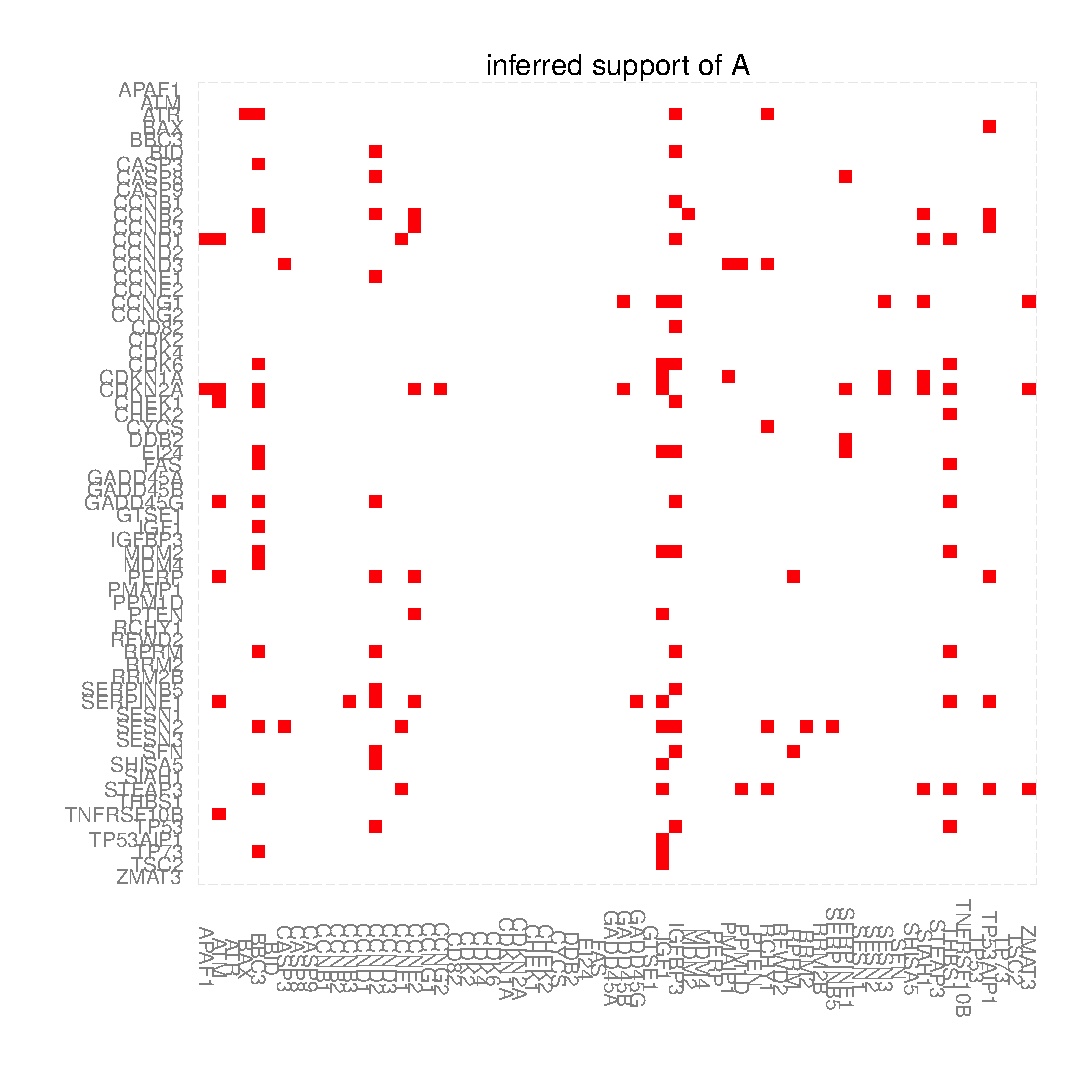
\includegraphics[scale=0.4, angle=0]{Ahat_support.eps}
&
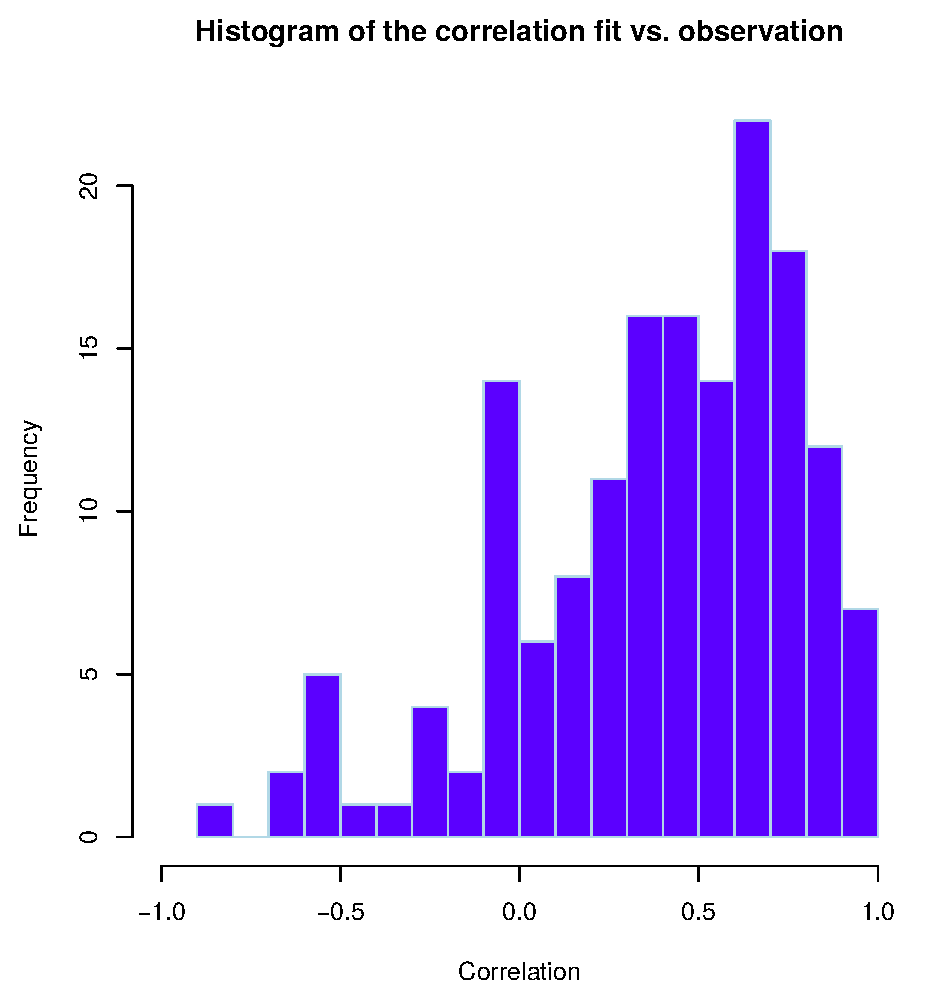
\includegraphics[scale=0.4, angle=0]{correlationFit2Obs.eps}
\\
\multicolumn{2}{c}{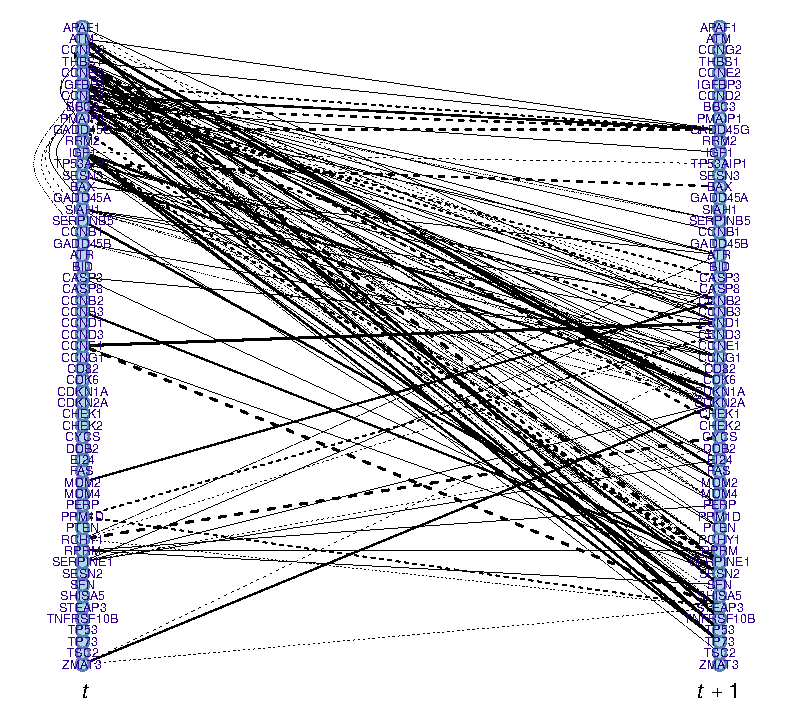
\includegraphics[scale=1.2, angle=0]{TSCG.eps}}  
\end{tabular}
\caption{Top row, left: the inferred support of $\mathbf{A}$; right: the histogram of gene-wise and cell line-wise correlation of fit and observation. Bottom panel: the time-series chain graph for the p53 signalling pathway.}
\label{fig:TSCG_supportA_fitHistogram}
\end{figure}
\afterpage{\clearpage}

The aforementioned `regulators' are known either to be pivotal to the p53 signalling pathway or to be involved in HPV-induced carcinogenesis. For instance, IGF1 (insulin-like growth factor 1) is a growth factor that regulates proliferation of both normal and cancer cells in an autocrine, paracrine \cite{Baxter2000} and potentially endocrine manner \cite{D'Ercole2001}. HPV transformed keratinocytes were found to be addicted to IGF1 signalling for survival, underlining the importance of this pathway for cervical cancer development \cite{Geiger2007}. IGFBP3, central to this signalling pathway, is transcriptionally regulated by p53 and (among others) suppresses proliferation and induces apoptosis (the process of programmed cell death). In our model lacking functional p53 due to presence of the HPV oncoprotein E6, IGFBP3 is down-regulated (data not shown) and, thus, does no longer inhibit carcinogenesis. Downregulation of THBS1, a potent angiogenesis inhibitor, was described before after expression of the viral oncogenes E6 and E7 in keratinocytes of different origins \citep{ToussaintSmith2004}. Lowered expression was also observed in cervical cancers \cite{Kodama2001}. 


With knowledge of their support less biased estimates of $\mathbf{A}$ and $\mathbf{\Omega}_{\varepsilon}$ are obtained by refitting them taking the support into account. Optimal penalty parameters are re-determined: $\lambda_a=2.55082$, $\lambda_{\omega}=0.00583$ (and confirmed by the contour plot the LOOCV log-likelihood surface, \cite{Supp2018}, Figure 3.30). Re-estimated parameters are visualized as a heatmap (\cite{Supp2018}, Figure 3.32). Using these estimates the time-series chain graph is constructed (Figure \ref{fig:TSCG_supportA_fitHistogram}). This is in line with the above suggested interpretation of `regulators'  and `regulatees'. 


Employing the re-estimated parameter $\mathbf{A}$, we study the fit ($\hat{\mathbf{Y}}_{\ast, i, t} = \hat{\mathbf{A}} \mathbf{Y}_{\ast, i, t-1}$) of the `regulatees' (genes explained by other genes). The fit is studied for all genes in the pathway. The result is summarized in Figure \ref{fig:TSCG_supportA_fitHistogram}. It displays the histogram of the Spearman correlations between the fit and the observations, cell line-wise. The histogram in Figure \ref{fig:TSCG_supportA_fitHistogram} is clearly skewed to the domain $[0,1]$. This indicates that the fit is generally reasonable. For a more tangible assessment of the fit it is displayed for several individual genes in Figure 3.34 \cite{Supp2018}.

\begin{figure}[t!]
\centering
\begin{tabular}{ccc}
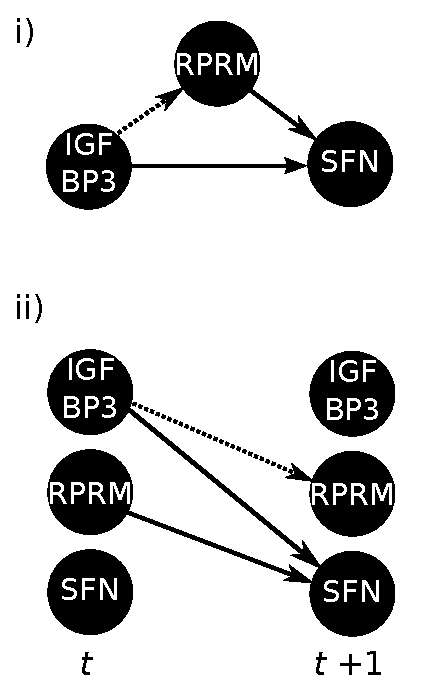
\includegraphics[scale=0.63, angle=0]{motif_incoherentFFL.eps}
& \mbox{ } \qquad \mbox{ } &
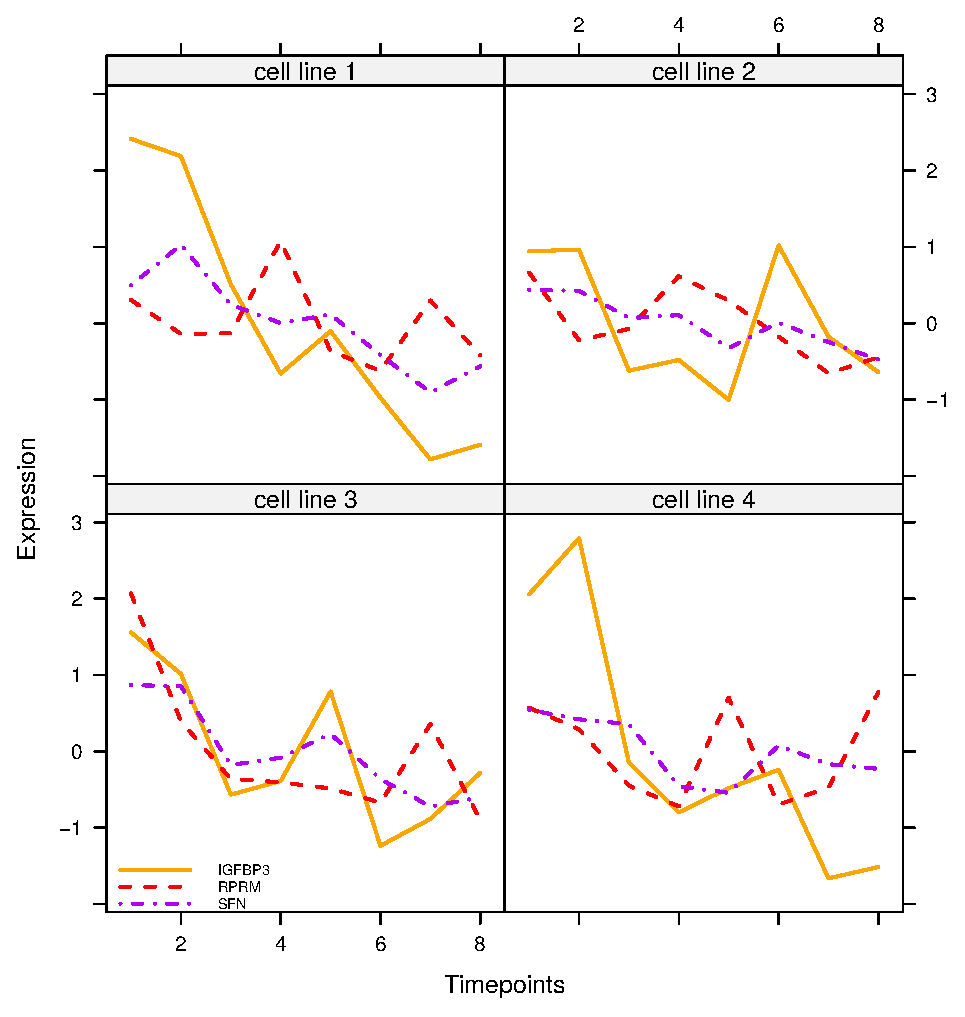
\includegraphics[scale=0.41, angle=0]{motif_incoherentFFL_data.eps}
\end{tabular}
\caption{Left panel, i): incoherent FFL motif formed by the gene-triple IGFBP3, RPRM and SFN. The solid (dashed) edge represent a positive (negative) effect. Left panel, ii): same as i) but `unrolled'. Right panel: gene expression data of the IGFBP3, RPRM and SFN genes over time in the four cell lines. }
\label{fig:motif_incoherentFFL}
\end{figure}
 \afterpage{\clearpage}


With final and less-biased estimates of the VAR(1) parameters at hand, we study the quantitative, dynamic implications of the model: what are the downstream effects of a change in expression levels of a gene? This can be done through impulse response analysis (confer Section \ref{sect:impulseResponse}). For each gene the column-wise average of the (absolute) impulse response on all other genes at the next time instance is calculated (Table 3.2, \cite{Supp2018}). This is a measure of a gene's driving force on the pathway's expression levels. The low and high impulse responses of the $\{\mbox{CCNG1, CGKN2A, SERPINE1, SESN2, STEAP3}\}$ and \\ $\{\mbox{IGF1, IGFBP3, BBC3, CCND2, THBS1}\}$ genes corroborate with their interpretations of `regulatees' and `regulators'. This is supported when evaluating the mutual information between each gene at time point $t$ and the whole pathway at the next time point (Table 3.2, \cite{Supp2018}). 

The downstream effects of a signal may be further elucidated through the decomposition of the covariance between the expression levels of two genes in terms of the paths connecting them in the time-series chain graph (as described in Section \ref{sect.pathDecomposition}). For illustration purposes consider the `regulator'-`regulatee' pair (IGF1, SESN2) at two contiguous time points. They are connected through two paths: a direct path $(Y_{\mbox{{\tiny IGF1}},t} \rightarrow Y_{\mbox{{\tiny SESN2}},t+1})$ and an indirect one through $Y_{\mbox{{\tiny IGF1}},t} \rightarrow Y_{\mbox{{\tiny RRM2}},t}\rightarrow Y_{\mbox{{\tiny SESN2}},t+1}$. The covariance of the (IGF1, SESN2) gene pair at contiguous time points may now be decomposed as: $\mbox{Cov}(Y_{\mbox{{\tiny IGF1}},t},Y_{\mbox{{\tiny SESN2}},t+1}) = (\boldsymbol{\Sigma}_{\varepsilon} \textbf{A}^\top)_{\mbox{{\tiny IGF1}}, \mbox{{\tiny SESN2}}} =  -0.05315 = -0.02203  - 0.03112$, in which the two summands on the right-hand side correspond to the direct and indirect path in the time-series chain graph. Based on the paths' contributions the indirect one dominates (surprisingly), but being of the same sign and (approximately) of the same size the direct path also contributes in the suppression of the expression levels of the SESN2 gene.


Another way to grasp the inferred networks of the p53 signalling pathway is to study its motifs. Motifs are small recurring network patterns and form the building blocks of pathways \cite{Alon2007}. It takes to far afield to study all motifs present in the inferred network (although it is relatively sparse) in depth. For the purpose of illustration we single out the feedforward loop (FFL), which appears in many gene systems \cite{Alon2007}. FFL motifs come in the coherent and incoherent variety: the latter connects two genes via two paths that have opposite effects (positive/activating and negative/repressing), while in the former both paths have the same effect. In an incohorent FFL motif found in the reconstructed time-series chain graph of the p53 signalling pathway gene IGFBP3 represses RPRM and activates SFN, while (to a lesser degree) RPRM stimulates SFN gene (Figure \ref{fig:motif_incoherentFFL}). IGFBP3 and RPRM thus affect SFN in opposite ways. In the extreme case, when the effect of the RPRM is equal to that of IGFBP3, this results (with a slight delay due to the time) in the repression of the SFN, reducing its expression levels to (virtually) zero (confer \cite{Alon2007}). In any case, the effect of IGFBP3 on SFN is moderated by that of RPRM (as is corroborated by the data (Figure \ref{fig:motif_incoherentFFL}).


\section{Conclusion}
The reconstruction of the time-series chain graph associated with a VAR(1) model from high-dimensional omics data was studied. To this end we presented a ridge penalized, full maximum likelihood estimation framework. The resulting estimator was simplified algebraically to ensure its computationally efficient evaluation from high-dimensional data. The estimator allows the incorporation of prior knowledge in two ways. First, the penalty of both VAR(1) model parameters includes a user-chosen target, representing a suggestion of the actual parameter value towards which the parameter is shrunken. Secondly, knowledge on the absence of certain cross-temporal and contemporaneous edges of the time-series chain graph may be included. Various novel ways to make use of the thus estimated  VAR(1) model were presented: \textit{i}) edge selection of the time-series chain graph from the estimated model, \textit{ii}) mutual information analysis across time points, and \textit{iii}) decomposition of the covariance between nodes across time points in terms of the paths of the time-series chain graph connecting them. Then, the proposed ridge estimation procedure was compared in simulation to a SCAD penalized estimator of the time-series chain graph. The ridge estimation procedure outperformed its SCAD counterpart in terms of loss and showed to be competitive in terms of specificity and sensitivity, in particular for small sample sizes (as is the prevalent experimental design for practice). Finally, the use of the presented methodology is illustrated on a time course experiment using an HPV-induced transformation cell line model.

Further biological questions to be (partially) answered using the high-dimensional omics data of the aforementioned cell line experiment require extensions of the proposed ridge estimation framework to more intricate vector autoregressive models. For instance, the full experiment also encompasses data from other molecular levels like DNA copy number and microRNA expression. Inclusion of these levels, both affecting mRNA expression, may be done within a VARX(1) model, a VAR(1) model with time-varying covariates (hence, the $X$ in VARX), which models the variation of mRNA expression over time by mRNA expression of the preceding time point and e.g. DNA copy number of the current time point. Another extension would address the fact that each cell line in the experiment had a different HPV inserted to initiate oncogenesis. This may lead to differences in the cell lines' time-series chain graphs. To detect such differences in regulatory architecture a VAR(1) model may be assumed per cell line and fitted with a fused ridge penalty \cite{Bilgrau2015}. Such a penalty fuses what is similar among the cell lines and preserves substantial differences among them. Future work will center around these and related topics to extract all relevant biological information from integrative time-course omics studies such as the cervical cancer one.

